%%Tracking
\input{data/tracking/qRobot1SlowTracking.txt}
\input{data/tracking/qRobot2SlowTracking.txt}
\input{data/tracking/qRobot3SlowTracking.txt}
\input{data/tracking/qRobot4SlowTracking.txt}
\input{data/tracking/qRobot5SlowTracking.txt}
\input{data/tracking/qRobot6SlowTracking.txt}
\input{data/tracking/qRobot7SlowTracking.txt}

\input{data/tracking/cameraPoseP0SlowTracking.txt}
\input{data/tracking/cameraPoseP1SlowTracking.txt}
\input{data/tracking/cameraPoseP2SlowTracking.txt}
\input{data/tracking/cameraPoseR0SlowTracking.txt}
\input{data/tracking/cameraPoseR1SlowTracking.txt}
\input{data/tracking/cameraPoseR2SlowTracking.txt}

\input{data/tracking/errorPoseXSlowTracking.txt}
\input{data/tracking/errorPoseYSlowTracking.txt}
\input{data/tracking/errorPoseXMediumTracking.txt}
\input{data/tracking/errorPoseYMediumTracking.txt}
\input{data/tracking/errorPoseXFastTracking.txt}
\input{data/tracking/errorPoseYFastTracking.txt}


\newcommand{\trackingSlowQRobotPlot}{
\label{plo:trackingQRobotPlot}
\begin{figure}[!ht]
\centering
	\tikzset{every mark/.append style={scale=0.5}}
	\begin{tikzpicture}
		\begin{axis}[height=9cm, width=\textwidth, grid=major,
		xlabel={Step},ylabel={rad}
		]	
			\addplot [color=Cyan, mark=o] coordinates {
				\trackingSlowQRobotDataA
			};
			\addlegendentry{q1}

			\addplot [color=DarkOrchid, mark=o] coordinates {
				\trackingSlowQRobotDataB
			};
			\addlegendentry{q2}
			
			\addplot [color=LimeGreen, mark=o] coordinates {
				\trackingSlowQRobotDataC
			};
			\addlegendentry{q3}
			
			\addplot [color=OrangeRed, mark=o] coordinates {
				\trackingSlowQRobotDataD
			};
			\addlegendentry{q4}
			
			\addplot [color=Goldenrod, mark=o] coordinates {
				\trackingSlowQRobotDataE
			};
			\addlegendentry{q5}
			
			\addplot [color=CarnationPink, mark=o] coordinates {
				\trackingSlowQRobotDataF
			};
			\addlegendentry{q6}

			\addplot [color=RoyalBlue, mark=o] coordinates {
				\trackingSlowQRobotDataG
			};
			\addlegendentry{q7}
		\end{axis}
	\end{tikzpicture}
	\caption{Robot's State while tracking the marker at slow speed.}
\end{figure}
}

\newcommand{\trackingSlowCameraPose}{
\label{plo:trackingSlowCameraPose}
\begin{figure}[!ht]
\centering
	\tikzset{every mark/.append style={scale=0.5}}
	\begin{tikzpicture} [spy using outlines=
	{circle, magnification=10, connect spies}
	]
		\begin{axis}[height=9cm, width=\textwidth, grid=major,
		xlabel={Step},ylabel={rad}
		]	
			\addplot [color=Cyan, mark=o] coordinates {
				\trackingSlowCameraPoseDataA
			};
			\addlegendentry{P0}

			\addplot [color=DarkOrchid, mark=o] coordinates {
				\trackingSlowCameraPoseDataB
			};
			\addlegendentry{P1}
			
			\addplot [color=LimeGreen, mark=o] coordinates {
				\trackingSlowCameraPoseDataC
			};
			\addlegendentry{P2}
			
			\addplot [color=OrangeRed, mark=o] coordinates {
				\trackingSlowCameraPoseDataD
			};
			\addlegendentry{R}
			
			\addplot [color=Goldenrod, mark=o] coordinates {
				\trackingSlowCameraPoseDataE
			};
			\addlegendentry{P}
			
			\addplot [color=CarnationPink, mark=o] coordinates {
				\trackingSlowCameraPoseDataF
			};
			\addlegendentry{Y}

			\coordinate (spypoint) at (axis cs:200,-0.31);
 			\coordinate (magnifyglass) at (axis cs:350,0.85);
		\end{axis}
		\spy [blue, size=2.0cm] on (spypoint) in node[fill=white] at (magnifyglass);
	\end{tikzpicture}
	\caption{Camera pose when tracking the marker at slow speed}
\end{figure}
}

\newcommand{\trackingErrorPlot}{
\label{plo:trackingErrorPlot}
\begin{figure}[!ht]
\centering
	\begin{tikzpicture}
		\begin{axis}[height=9cm, width=\textwidth, grid=major,
		xlabel={Step},ylabel={rad}
		]	
			\addplot [color=Cyan, mark=o] coordinates {
				\trackingSlowErrorPoseDataX
			};
			\addlegendentry{Slow Error X}

			\addplot [color=DarkOrchid, mark=o] coordinates {
				\trackingSlowErrorPoseDataY
			};
			\addlegendentry{Slow Error Y}
			
			\addplot [color=LimeGreen, mark=o] coordinates {
				\trackingMediumErrorPoseDataX
			};
			\addlegendentry{Medium Error X}
			
			\addplot [color=OrangeRed, mark=o] coordinates {
				\trackingMediumErrorPoseDataY
			};
			\addlegendentry{Medium Error Y}
			
			\addplot [color=Goldenrod, mark=o] coordinates {
				\trackingFastErrorPoseDataX
			};
			\addlegendentry{Fast Error X}
			
			\addplot [color=CarnationPink, mark=o] coordinates {
				\trackingFastErrorPoseDataY
			};
			\addlegendentry{Fast Error Y}
		\end{axis}
	\end{tikzpicture}
	\caption{Error in the X and Y coordinates. Tracking marker at different speeds}
\end{figure}
}

\providecommand{\errorTrackingPlot}{
\begin{figure}[!ht]
	\centering
	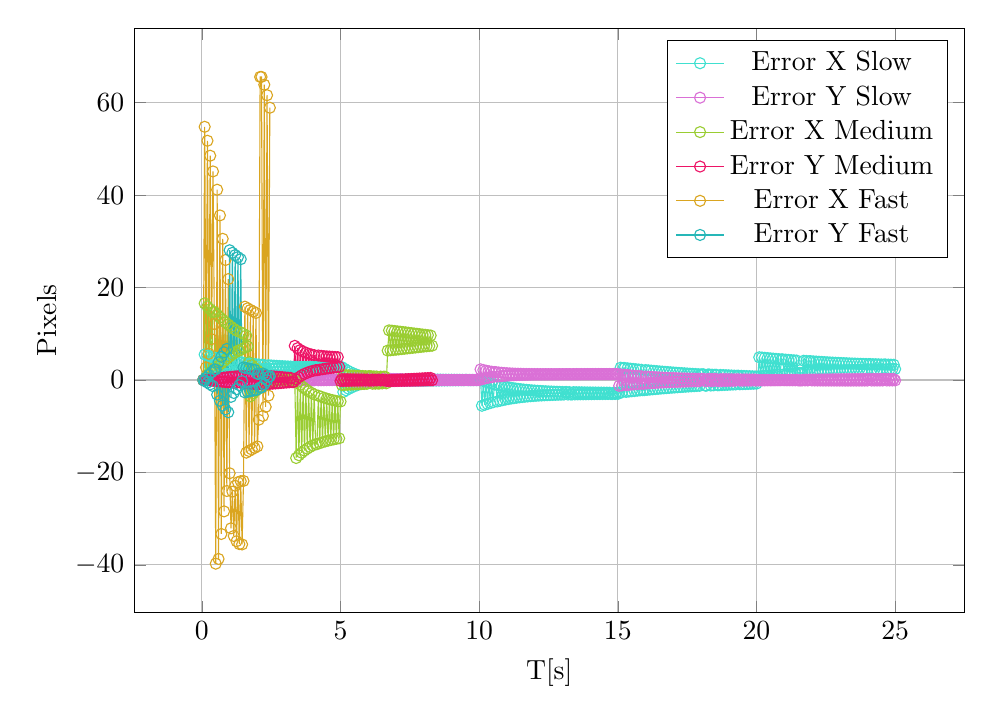
\begin{tikzpicture}
		\begin{axis}[height=9cm, width=\textwidth, grid=major,
		xlabel={T[s]},ylabel={Pixels}
		]
			\addplot [color=Turquoise, mark=o] coordinates {
				(0.050,-0.000)
				(0.100,5.530)
				(0.150,0.222)
				(0.200,5.317)
				(0.250,0.426)
				(0.300,5.120)
				(0.350,0.615)
				(0.400,4.938)
				(0.450,0.790)
				(0.500,4.770)
				(0.550,0.952)
				(0.600,0.952)
				(0.650,4.616)
				(0.700,1.100)
				(0.750,4.472)
				(0.800,1.239)
				(0.850,4.339)
				(0.900,1.367)
				(0.950,4.216)
				(1.000,4.216)
				(1.050,1.486)
				(1.100,4.099)
				(1.150,1.598)
				(1.200,3.991)
				(1.250,1.702)
				(1.300,1.702)
				(1.350,3.893)
				(1.400,1.797)
				(1.450,3.800)
				(1.500,1.887)
				(1.550,3.713)
				(1.600,1.971)
				(1.650,3.632)
				(1.700,2.050)
				(1.750,3.556)
				(1.800,2.123)
				(1.850,3.485)
				(1.900,2.191)
				(1.950,3.419)
				(2.000,2.254)
				(2.050,3.358)
				(2.100,2.313)
				(2.150,3.300)
				(2.200,2.369)
				(2.250,3.247)
				(2.300,2.420)
				(2.350,2.420)
				(2.400,3.200)
				(2.450,2.466)
				(2.500,3.153)
				(2.550,2.511)
				(2.600,3.110)
				(2.650,2.552)
				(2.700,3.070)
				(2.750,2.590)
				(2.800,3.033)
				(2.850,2.626)
				(2.900,2.999)
				(2.950,2.658)
				(3.000,2.967)
				(3.050,2.688)
				(3.100,2.939)
				(3.150,2.715)
				(3.200,2.913)
				(3.250,2.740)
				(3.300,2.889)
				(3.350,2.762)
				(3.400,2.868)
				(3.450,2.782)
				(3.500,2.849)
				(3.550,2.800)
				(3.600,2.832)
				(3.650,2.815)
				(3.700,2.817)
				(3.750,2.829)
				(3.800,2.804)
				(3.850,2.804)
				(3.900,2.844)
				(3.950,2.790)
				(4.000,2.854)
				(4.050,2.780)
				(4.100,2.862)
				(4.150,2.862)
				(4.200,2.776)
				(4.250,2.865)
				(4.300,2.770)
				(4.350,2.870)
				(4.400,2.765)
				(4.450,2.874)
				(4.500,2.761)
				(4.550,2.877)
				(4.600,2.759)
				(4.650,2.879)
				(4.700,2.757)
				(4.750,2.879)
				(4.800,2.757)
				(4.850,2.879)
				(4.900,2.757)
				(4.950,2.878)
				(5.000,2.758)
				(5.050,2.791)
				(5.100,-2.593)
				(5.150,2.403)
				(5.200,-2.225)
				(5.250,2.055)
				(5.300,-1.896)
				(5.350,1.744)
				(5.400,-1.602)
				(5.450,1.467)
				(5.500,-1.341)
				(5.550,1.222)
				(5.600,-1.111)
				(5.650,1.006)
				(5.700,-0.908)
				(5.750,0.816)
				(5.800,-0.731)
				(5.850,0.651)
				(5.900,-0.577)
				(5.950,0.508)
				(6.000,-0.444)
				(6.050,0.384)
				(6.100,-0.329)
				(6.150,0.278)
				(6.200,-0.232)
				(6.250,0.189)
				(6.300,-0.149)
				(6.350,0.113)
				(6.400,-0.080)
				(6.450,0.050)
				(6.500,-0.023)
				(6.550,-0.002)
				(6.600,0.024)
				(6.650,-0.044)
				(6.700,0.062)
				(6.750,-0.078)
				(6.800,0.092)
				(6.850,-0.105)
				(6.900,0.116)
				(6.950,-0.125)
				(7.000,0.133)
				(7.050,-0.140)
				(7.100,0.145)
				(7.150,-0.150)
				(7.200,0.153)
				(7.250,-0.156)
				(7.300,-0.156)
				(7.350,0.158)
				(7.400,-0.159)
				(7.450,0.159)
				(7.500,-0.159)
				(7.550,-0.159)
				(7.600,0.158)
				(7.650,-0.157)
				(7.700,0.155)
				(7.750,-0.153)
				(7.800,0.151)
				(7.850,-0.148)
				(7.900,0.145)
				(7.950,-0.142)
				(8.000,0.139)
				(8.050,-0.135)
				(8.100,0.132)
				(8.150,-0.128)
				(8.200,0.124)
				(8.250,-0.120)
				(8.300,0.116)
				(8.350,-0.112)
				(8.400,0.108)
				(8.450,-0.104)
				(8.500,0.100)
				(8.550,-0.096)
				(8.600,0.092)
				(8.650,-0.089)
				(8.700,0.085)
				(8.750,-0.081)
				(8.800,0.078)
				(8.850,-0.074)
				(8.900,0.071)
				(8.950,-0.067)
				(9.000,0.064)
				(9.050,-0.061)
				(9.100,0.058)
				(9.150,-0.055)
				(9.200,0.052)
				(9.250,-0.049)
				(9.300,0.046)
				(9.350,-0.044)
				(9.400,0.041)
				(9.450,-0.039)
				(9.500,0.036)
				(9.550,0.036)
				(9.600,-0.034)
				(9.650,0.032)
				(9.700,-0.030)
				(9.750,0.028)
				(9.800,-0.026)
				(9.850,0.025)
				(9.900,-0.023)
				(9.950,0.021)
				(10.000,-0.020)
				(10.050,0.001)
				(10.100,-5.562)
				(10.150,-0.214)
				(10.200,-5.354)
				(10.250,-0.418)
				(10.300,-5.158)
				(10.350,-0.610)
				(10.400,-4.974)
				(10.450,-0.790)
				(10.500,-4.802)
				(10.550,-0.957)
				(10.600,-0.957)
				(10.650,-4.639)
				(10.700,-1.115)
				(10.750,-4.491)
				(10.800,-1.259)
				(10.850,-4.355)
				(10.900,-1.392)
				(10.950,-4.230)
				(11.000,-1.514)
				(11.050,-4.115)
				(11.100,-1.625)
				(11.150,-4.011)
				(11.200,-1.727)
				(11.250,-3.915)
				(11.300,-1.820)
				(11.350,-3.828)
				(11.400,-1.905)
				(11.450,-3.749)
				(11.500,-1.983)
				(11.550,-3.678)
				(11.600,-2.053)
				(11.650,-3.613)
				(11.700,-2.117)
				(11.750,-3.554)
				(11.800,-2.175)
				(11.850,-3.500)
				(11.900,-2.228)
				(11.950,-3.452)
				(12.000,-2.276)
				(12.050,-3.408)
				(12.100,-2.320)
				(12.150,-3.368)
				(12.200,-2.360)
				(12.250,-3.332)
				(12.300,-2.396)
				(12.350,-3.300)
				(12.400,-2.429)
				(12.450,-3.270)
				(12.500,-2.459)
				(12.550,-3.244)
				(12.600,-2.486)
				(12.650,-3.220)
				(12.700,-2.511)
				(12.750,-3.198)
				(12.800,-2.534)
				(12.850,-3.178)
				(12.900,-2.555)
				(12.950,-3.160)
				(13.000,-2.574)
				(13.050,-3.144)
				(13.100,-2.591)
				(13.150,-2.591)
				(13.200,-3.130)
				(13.250,-2.607)
				(13.300,-3.117)
				(13.350,-3.117)
				(13.400,-2.623)
				(13.450,-3.104)
				(13.500,-2.636)
				(13.550,-3.094)
				(13.600,-2.648)
				(13.650,-3.084)
				(13.700,-2.659)
				(13.750,-3.075)
				(13.800,-2.670)
				(13.850,-3.067)
				(13.900,-2.679)
				(13.950,-3.059)
				(14.000,-2.688)
				(14.050,-3.053)
				(14.100,-2.696)
				(14.150,-3.046)
				(14.200,-2.704)
				(14.250,-3.040)
				(14.300,-2.711)
				(14.350,-3.035)
				(14.400,-2.718)
				(14.450,-3.030)
				(14.500,-2.724)
				(14.550,-3.026)
				(14.600,-2.730)
				(14.650,-3.022)
				(14.700,-2.736)
				(14.750,-3.018)
				(14.800,-3.018)
				(14.850,-2.743)
				(14.900,-3.013)
				(14.950,-2.748)
				(15.000,-3.009)
				(15.050,-2.713)
				(15.100,2.676)
				(15.150,-2.638)
				(15.200,2.603)
				(15.250,2.603)
				(15.300,-2.566)
				(15.350,2.533)
				(15.400,-2.499)
				(15.450,2.466)
				(15.500,-2.433)
				(15.550,2.401)
				(15.600,-2.369)
				(15.650,2.338)
				(15.700,-2.306)
				(15.750,2.276)
				(15.800,-2.245)
				(15.850,2.215)
				(15.900,-2.185)
				(15.950,-2.185)
				(16.000,2.156)
				(16.050,-2.126)
				(16.100,2.097)
				(16.150,-2.068)
				(16.200,2.039)
				(16.250,-2.011)
				(16.300,1.983)
				(16.350,-1.956)
				(16.400,1.929)
				(16.450,-1.902)
				(16.500,1.876)
				(16.550,-1.849)
				(16.600,1.824)
				(16.650,-1.798)
				(16.700,1.773)
				(16.750,-1.749)
				(16.800,1.724)
				(16.850,-1.700)
				(16.900,1.677)
				(16.950,-1.653)
				(17.000,1.630)
				(17.050,-1.607)
				(17.100,1.585)
				(17.150,-1.563)
				(17.200,1.541)
				(17.250,-1.520)
				(17.300,1.498)
				(17.350,-1.477)
				(17.400,1.457)
				(17.450,-1.436)
				(17.500,1.416)
				(17.550,-1.396)
				(17.600,1.377)
				(17.650,-1.358)
				(17.700,1.339)
				(17.750,-1.320)
				(17.800,1.301)
				(17.850,-1.283)
				(17.900,1.265)
				(17.950,-1.247)
				(18.000,1.230)
				(18.050,1.230)
				(18.100,1.230)
				(18.150,-1.213)
				(18.200,-1.213)
				(18.250,1.196)
				(18.300,1.196)
				(18.350,-1.179)
				(18.400,1.163)
				(18.450,-1.147)
				(18.500,1.131)
				(18.550,1.131)
				(18.600,-1.115)
				(18.650,-1.115)
				(18.700,1.100)
				(18.750,-1.085)
				(18.800,1.070)
				(18.850,-1.055)
				(18.900,1.040)
				(18.950,-1.026)
				(19.000,1.012)
				(19.050,-0.998)
				(19.100,0.984)
				(19.150,-0.970)
				(19.200,0.957)
				(19.250,-0.943)
				(19.300,0.930)
				(19.350,0.930)
				(19.400,-0.917)
				(19.450,0.905)
				(19.500,-0.892)
				(19.550,0.880)
				(19.600,-0.867)
				(19.650,0.855)
				(19.700,-0.844)
				(19.750,0.832)
				(19.800,-0.820)
				(19.850,0.809)
				(19.900,-0.798)
				(19.950,0.787)
				(20.000,-0.776)
				(20.050,0.766)
				(20.100,4.924)
				(20.150,0.826)
				(20.200,4.864)
				(20.250,0.885)
				(20.300,4.805)
				(20.350,0.943)
				(20.400,4.747)
				(20.450,1.000)
				(20.500,4.690)
				(20.550,1.057)
				(20.600,4.634)
				(20.650,1.112)
				(20.700,4.579)
				(20.750,1.166)
				(20.800,4.525)
				(20.850,1.219)
				(20.900,4.472)
				(20.950,4.472)
				(21.000,1.272)
				(21.050,4.418)
				(21.100,1.324)
				(21.150,4.365)
				(21.200,1.375)
				(21.250,4.314)
				(21.300,1.425)
				(21.350,4.264)
				(21.400,1.474)
				(21.450,4.216)
				(21.500,1.522)
				(21.550,1.522)
				(21.600,1.522)
				(21.650,1.522)
				(21.700,4.175)
				(21.750,1.563)
				(21.800,4.129)
				(21.850,1.607)
				(21.900,4.085)
				(21.950,4.085)
				(22.000,1.651)
				(22.050,4.040)
				(22.100,1.693)
				(22.150,3.998)
				(22.200,1.734)
				(22.250,3.957)
				(22.300,1.774)
				(22.350,3.918)
				(22.400,1.811)
				(22.450,3.880)
				(22.500,1.848)
				(22.550,3.844)
				(22.600,1.883)
				(22.650,3.809)
				(22.700,1.916)
				(22.750,3.776)
				(22.800,1.948)
				(22.850,3.744)
				(22.900,1.978)
				(22.950,3.714)
				(23.000,2.008)
				(23.050,3.685)
				(23.100,2.036)
				(23.150,3.657)
				(23.200,2.062)
				(23.250,3.630)
				(23.300,2.088)
				(23.350,3.604)
				(23.400,2.112)
				(23.450,3.580)
				(23.500,2.135)
				(23.550,3.556)
				(23.600,2.157)
				(23.650,3.534)
				(23.700,2.179)
				(23.750,3.512)
				(23.800,2.199)
				(23.850,3.492)
				(23.900,2.218)
				(23.950,3.472)
				(24.000,2.237)
				(24.050,3.453)
				(24.100,3.453)
				(24.150,2.257)
				(24.200,3.430)
				(24.250,2.275)
				(24.300,3.412)
				(24.350,2.292)
				(24.400,3.395)
				(24.450,2.308)
				(24.500,3.378)
				(24.550,2.324)
				(24.600,3.362)
				(24.650,3.362)
				(24.700,2.342)
				(24.750,3.341)
				(24.800,2.357)
				(24.850,3.325)
				(24.900,2.372)
				(24.950,3.310)
				(25.000,2.386)

			};
			\addlegendentry{Error X Slow}

			\addplot [color=Orchid, mark=o] coordinates {
				(0.050,0.000)
				(0.100,-0.000)
				(0.150,0.003)
				(0.200,-0.002)
				(0.250,0.008)
				(0.300,-0.006)
				(0.350,0.015)
				(0.400,-0.011)
				(0.450,0.022)
				(0.500,-0.018)
				(0.550,0.031)
				(0.600,0.031)
				(0.650,-0.021)
				(0.700,0.039)
				(0.750,-0.029)
				(0.800,0.049)
				(0.850,-0.037)
				(0.900,0.059)
				(0.950,-0.046)
				(1.000,-0.046)
				(1.050,0.071)
				(1.100,-0.056)
				(1.150,0.082)
				(1.200,-0.065)
				(1.250,0.093)
				(1.300,0.093)
				(1.350,-0.070)
				(1.400,0.101)
				(1.450,-0.079)
				(1.500,0.111)
				(1.550,-0.086)
				(1.600,0.121)
				(1.650,-0.094)
				(1.700,0.129)
				(1.750,-0.100)
				(1.800,0.137)
				(1.850,-0.106)
				(1.900,0.145)
				(1.950,-0.111)
				(2.000,0.151)
				(2.050,-0.115)
				(2.100,0.157)
				(2.150,-0.118)
				(2.200,0.161)
				(2.250,-0.120)
				(2.300,0.165)
				(2.350,0.165)
				(2.400,-0.119)
				(2.450,0.167)
				(2.500,-0.120)
				(2.550,0.170)
				(2.600,-0.121)
				(2.650,0.171)
				(2.700,-0.120)
				(2.750,0.172)
				(2.800,-0.119)
				(2.850,0.173)
				(2.900,-0.117)
				(2.950,0.172)
				(3.000,-0.114)
				(3.050,0.171)
				(3.100,-0.110)
				(3.150,0.169)
				(3.200,-0.106)
				(3.250,0.167)
				(3.300,-0.102)
				(3.350,0.164)
				(3.400,-0.096)
				(3.450,0.160)
				(3.500,-0.091)
				(3.550,0.157)
				(3.600,-0.085)
				(3.650,0.153)
				(3.700,-0.079)
				(3.750,0.148)
				(3.800,-0.072)
				(3.850,-0.072)
				(3.900,0.146)
				(3.950,-0.066)
				(4.000,0.141)
				(4.050,-0.059)
				(4.100,0.136)
				(4.150,0.136)
				(4.200,-0.050)
				(4.250,0.129)
				(4.300,-0.042)
				(4.350,0.124)
				(4.400,-0.035)
				(4.450,0.119)
				(4.500,-0.028)
				(4.550,0.114)
				(4.600,-0.021)
				(4.650,0.109)
				(4.700,-0.014)
				(4.750,0.104)
				(4.800,-0.007)
				(4.850,0.100)
				(4.900,-0.001)
				(4.950,0.096)
				(5.000,0.006)
				(5.050,-0.059)
				(5.100,0.107)
				(5.150,-0.150)
				(5.200,0.188)
				(5.250,-0.222)
				(5.300,0.252)
				(5.350,-0.277)
				(5.400,0.300)
				(5.450,-0.319)
				(5.500,0.335)
				(5.550,-0.348)
				(5.600,0.359)
				(5.650,-0.367)
				(5.700,0.374)
				(5.750,-0.378)
				(5.800,0.381)
				(5.850,-0.382)
				(5.900,0.381)
				(5.950,-0.379)
				(6.000,0.377)
				(6.050,-0.373)
				(6.100,0.368)
				(6.150,-0.362)
				(6.200,0.355)
				(6.250,-0.348)
				(6.300,0.341)
				(6.350,-0.333)
				(6.400,0.324)
				(6.450,-0.315)
				(6.500,0.306)
				(6.550,-0.297)
				(6.600,0.287)
				(6.650,-0.278)
				(6.700,0.268)
				(6.750,-0.259)
				(6.800,0.249)
				(6.850,-0.240)
				(6.900,0.230)
				(6.950,-0.221)
				(7.000,0.212)
				(7.050,-0.203)
				(7.100,0.194)
				(7.150,-0.185)
				(7.200,0.176)
				(7.250,-0.168)
				(7.300,-0.168)
				(7.350,0.160)
				(7.400,-0.152)
				(7.450,0.144)
				(7.500,-0.137)
				(7.550,-0.137)
				(7.600,0.130)
				(7.650,-0.123)
				(7.700,0.116)
				(7.750,-0.110)
				(7.800,0.104)
				(7.850,-0.098)
				(7.900,0.092)
				(7.950,-0.087)
				(8.000,0.081)
				(8.050,-0.076)
				(8.100,0.071)
				(8.150,-0.067)
				(8.200,0.062)
				(8.250,-0.058)
				(8.300,0.054)
				(8.350,-0.051)
				(8.400,0.047)
				(8.450,-0.044)
				(8.500,0.040)
				(8.550,-0.037)
				(8.600,0.034)
				(8.650,-0.032)
				(8.700,0.029)
				(8.750,-0.027)
				(8.800,0.024)
				(8.850,-0.022)
				(8.900,0.020)
				(8.950,-0.018)
				(9.000,0.017)
				(9.050,-0.015)
				(9.100,0.013)
				(9.150,-0.012)
				(9.200,0.011)
				(9.250,-0.009)
				(9.300,0.008)
				(9.350,-0.007)
				(9.400,0.006)
				(9.450,-0.005)
				(9.500,0.004)
				(9.550,0.004)
				(9.600,-0.003)
				(9.650,0.003)
				(9.700,-0.002)
				(9.750,0.002)
				(9.800,-0.001)
				(9.850,0.000)
				(9.900,-0.000)
				(9.950,-0.000)
				(10.000,0.001)
				(10.050,2.316)
				(10.100,0.173)
				(10.150,2.159)
				(10.200,0.323)
				(10.250,2.022)
				(10.300,0.453)
				(10.350,1.905)
				(10.400,0.564)
				(10.450,1.804)
				(10.500,0.661)
				(10.550,1.717)
				(10.600,1.717)
				(10.650,0.750)
				(10.700,1.641)
				(10.750,0.821)
				(10.800,1.579)
				(10.850,0.882)
				(10.900,1.526)
				(10.950,0.934)
				(11.000,1.481)
				(11.050,0.978)
				(11.100,1.443)
				(11.150,1.016)
				(11.200,1.411)
				(11.250,1.048)
				(11.300,1.384)
				(11.350,1.076)
				(11.400,1.362)
				(11.450,1.099)
				(11.500,1.343)
				(11.550,1.119)
				(11.600,1.328)
				(11.650,1.137)
				(11.700,1.315)
				(11.750,1.151)
				(11.800,1.305)
				(11.850,1.164)
				(11.900,1.297)
				(11.950,1.175)
				(12.000,1.290)
				(12.050,1.184)
				(12.100,1.285)
				(12.150,1.192)
				(12.200,1.281)
				(12.250,1.199)
				(12.300,1.278)
				(12.350,1.205)
				(12.400,1.275)
				(12.450,1.211)
				(12.500,1.274)
				(12.550,1.216)
				(12.600,1.273)
				(12.650,1.220)
				(12.700,1.273)
				(12.750,1.224)
				(12.800,1.273)
				(12.850,1.227)
				(12.900,1.273)
				(12.950,1.230)
				(13.000,1.274)
				(13.050,1.233)
				(13.100,1.275)
				(13.150,1.275)
				(13.200,1.240)
				(13.250,1.275)
				(13.300,1.242)
				(13.350,1.242)
				(13.400,1.279)
				(13.450,1.244)
				(13.500,1.280)
				(13.550,1.246)
				(13.600,1.282)
				(13.650,1.248)
				(13.700,1.284)
				(13.750,1.251)
				(13.800,1.285)
				(13.850,1.253)
				(13.900,1.287)
				(13.950,1.256)
				(14.000,1.289)
				(14.050,1.258)
				(14.100,1.290)
				(14.150,1.261)
				(14.200,1.292)
				(14.250,1.263)
				(14.300,1.294)
				(14.350,1.266)
				(14.400,1.296)
				(14.450,1.268)
				(14.500,1.297)
				(14.550,1.271)
				(14.600,1.299)
				(14.650,1.273)
				(14.700,1.301)
				(14.750,1.276)
				(14.800,1.276)
				(14.850,1.304)
				(14.900,1.279)
				(14.950,1.306)
				(15.000,1.282)
				(15.050,-1.244)
				(15.100,1.208)
				(15.150,-1.173)
				(15.200,1.138)
				(15.250,1.138)
				(15.300,-1.106)
				(15.350,1.075)
				(15.400,-1.044)
				(15.450,1.014)
				(15.500,-0.986)
				(15.550,0.957)
				(15.600,-0.930)
				(15.650,0.904)
				(15.700,-0.878)
				(15.750,0.853)
				(15.800,-0.829)
				(15.850,0.806)
				(15.900,-0.783)
				(15.950,-0.783)
				(16.000,0.760)
				(16.050,-0.738)
				(16.100,0.717)
				(16.150,-0.696)
				(16.200,0.676)
				(16.250,-0.657)
				(16.300,0.638)
				(16.350,-0.619)
				(16.400,0.601)
				(16.450,-0.584)
				(16.500,0.567)
				(16.550,-0.551)
				(16.600,0.535)
				(16.650,-0.520)
				(16.700,0.505)
				(16.750,-0.491)
				(16.800,0.476)
				(16.850,-0.463)
				(16.900,0.450)
				(16.950,-0.437)
				(17.000,0.424)
				(17.050,-0.412)
				(17.100,0.400)
				(17.150,-0.389)
				(17.200,0.378)
				(17.250,-0.367)
				(17.300,0.357)
				(17.350,-0.347)
				(17.400,0.337)
				(17.450,-0.327)
				(17.500,0.318)
				(17.550,-0.309)
				(17.600,0.300)
				(17.650,-0.292)
				(17.700,0.283)
				(17.750,-0.275)
				(17.800,0.268)
				(17.850,-0.260)
				(17.900,0.253)
				(17.950,-0.246)
				(18.000,0.239)
				(18.050,0.239)
				(18.100,0.239)
				(18.150,-0.232)
				(18.200,-0.232)
				(18.250,0.226)
				(18.300,0.226)
				(18.350,-0.220)
				(18.400,0.214)
				(18.450,-0.208)
				(18.500,0.202)
				(18.550,0.202)
				(18.600,-0.197)
				(18.650,-0.197)
				(18.700,0.192)
				(18.750,-0.186)
				(18.800,0.181)
				(18.850,-0.176)
				(18.900,0.172)
				(18.950,-0.167)
				(19.000,0.162)
				(19.050,-0.158)
				(19.100,0.154)
				(19.150,-0.150)
				(19.200,0.146)
				(19.250,-0.142)
				(19.300,0.138)
				(19.350,0.138)
				(19.400,-0.134)
				(19.450,0.131)
				(19.500,-0.127)
				(19.550,0.124)
				(19.600,-0.121)
				(19.650,0.118)
				(19.700,-0.115)
				(19.750,0.112)
				(19.800,-0.109)
				(19.850,0.106)
				(19.900,-0.103)
				(19.950,0.100)
				(20.000,-0.098)
				(20.050,0.002)
				(20.100,-0.090)
				(20.150,-0.001)
				(20.200,-0.082)
				(20.250,-0.005)
				(20.300,-0.073)
				(20.350,-0.010)
				(20.400,-0.064)
				(20.450,-0.014)
				(20.500,-0.054)
				(20.550,-0.020)
				(20.600,-0.044)
				(20.650,-0.025)
				(20.700,-0.034)
				(20.750,-0.031)
				(20.800,-0.023)
				(20.850,-0.037)
				(20.900,-0.013)
				(20.950,-0.013)
				(21.000,-0.041)
				(21.050,-0.002)
				(21.100,-0.047)
				(21.150,0.009)
				(21.200,-0.054)
				(21.250,0.020)
				(21.300,-0.060)
				(21.350,0.031)
				(21.400,-0.066)
				(21.450,0.041)
				(21.500,-0.071)
				(21.550,-0.071)
				(21.600,-0.071)
				(21.650,-0.071)
				(21.700,0.061)
				(21.750,-0.077)
				(21.800,0.071)
				(21.850,-0.083)
				(21.900,0.081)
				(21.950,0.081)
				(22.000,-0.086)
				(22.050,0.091)
				(22.100,-0.092)
				(22.150,0.100)
				(22.200,-0.096)
				(22.250,0.110)
				(22.300,-0.101)
				(22.350,0.118)
				(22.400,-0.104)
				(22.450,0.126)
				(22.500,-0.108)
				(22.550,0.134)
				(22.600,-0.111)
				(22.650,0.142)
				(22.700,-0.113)
				(22.750,0.149)
				(22.800,-0.116)
				(22.850,0.155)
				(22.900,-0.117)
				(22.950,0.161)
				(23.000,-0.119)
				(23.050,0.167)
				(23.100,-0.119)
				(23.150,0.172)
				(23.200,-0.120)
				(23.250,0.177)
				(23.300,-0.120)
				(23.350,0.182)
				(23.400,-0.120)
				(23.450,0.186)
				(23.500,-0.119)
				(23.550,0.190)
				(23.600,-0.118)
				(23.650,0.193)
				(23.700,-0.117)
				(23.750,0.197)
				(23.800,-0.116)
				(23.850,0.200)
				(23.900,-0.114)
				(23.950,0.202)
				(24.000,-0.112)
				(24.050,0.205)
				(24.100,0.205)
				(24.150,-0.108)
				(24.200,0.207)
				(24.250,-0.105)
				(24.300,0.209)
				(24.350,-0.103)
				(24.400,0.210)
				(24.450,-0.100)
				(24.500,0.212)
				(24.550,-0.096)
				(24.600,0.213)
				(24.650,0.213)
				(24.700,-0.091)
				(24.750,0.214)
				(24.800,-0.087)
				(24.850,0.215)
				(24.900,-0.084)
				(24.950,0.215)
				(25.000,-0.080)

			};
			\addlegendentry{Error Y Slow}

			\addplot [color=YellowGreen, mark=o] coordinates {
				(0.050,-0.000)
				(0.100,16.580)
				(0.150,0.676)
				(0.200,15.921)
				(0.250,1.310)
				(0.300,15.301)
				(0.350,1.909)
				(0.400,14.714)
				(0.450,14.714)
				(0.500,2.479)
				(0.550,14.119)
				(0.600,3.048)
				(0.650,13.556)
				(0.700,3.592)
				(0.750,13.016)
				(0.800,4.113)
				(0.850,12.499)
				(0.900,4.611)
				(0.950,12.005)
				(1.000,5.085)
				(1.050,11.535)
				(1.100,5.536)
				(1.150,11.090)
				(1.200,5.959)
				(1.250,10.672)
				(1.300,6.355)
				(1.350,6.355)
				(1.400,10.324)
				(1.450,6.692)
				(1.500,9.959)
				(1.550,7.032)
				(1.600,9.629)
				(1.650,7.261)
				(1.700,3.877)
				(1.750,-3.526)
				(1.800,3.192)
				(1.850,-2.886)
				(1.900,2.597)
				(1.950,-2.333)
				(2.000,2.085)
				(2.050,-1.857)
				(2.100,1.645)
				(2.150,-1.450)
				(2.200,1.269)
				(2.250,-1.104)
				(2.300,0.952)
				(2.350,-0.812)
				(2.400,0.684)
				(2.450,0.684)
				(2.500,-0.568)
				(2.550,0.461)
				(2.600,-0.365)
				(2.650,0.277)
				(2.700,-0.198)
				(2.750,0.127)
				(2.800,-0.064)
				(2.850,0.007)
				(2.900,0.044)
				(2.950,-0.089)
				(3.000,0.128)
				(3.050,-0.162)
				(3.100,0.192)
				(3.150,-0.218)
				(3.200,0.240)
				(3.250,-0.258)
				(3.300,-0.258)
				(3.350,0.236)
				(3.400,-16.870)
				(3.450,-0.420)
				(3.500,-16.270)
				(3.550,-1.009)
				(3.600,-15.735)
				(3.650,-1.534)
				(3.700,-15.261)
				(3.750,-2.001)
				(3.800,-14.844)
				(3.850,-2.415)
				(3.900,-14.477)
				(3.950,-2.780)
				(4.000,-14.156)
				(4.050,-3.103)
				(4.100,-13.875)
				(4.150,-13.875)
				(4.200,-3.391)
				(4.250,-13.652)
				(4.300,-3.621)
				(4.350,-13.453)
				(4.400,-3.827)
				(4.450,-13.276)
				(4.500,-4.013)
				(4.550,-13.118)
				(4.600,-4.181)
				(4.650,-12.975)
				(4.700,-4.335)
				(4.750,-12.844)
				(4.800,-4.477)
				(4.850,-12.723)
				(4.900,-4.610)
				(4.950,-12.611)
				(5.000,-4.653)
				(5.050,-1.091)
				(5.100,1.074)
				(5.150,-1.058)
				(5.200,1.041)
				(5.250,-1.026)
				(5.300,1.010)
				(5.350,-0.994)
				(5.400,0.979)
				(5.450,-0.964)
				(5.500,0.949)
				(5.550,-0.935)
				(5.600,0.921)
				(5.650,-0.907)
				(5.700,0.893)
				(5.750,-0.879)
				(5.800,0.866)
				(5.850,-0.853)
				(5.900,0.840)
				(5.950,-0.827)
				(6.000,0.815)
				(6.050,0.815)
				(6.100,0.815)
				(6.150,-0.802)
				(6.200,0.790)
				(6.250,-0.778)
				(6.300,0.766)
				(6.350,-0.754)
				(6.400,-0.754)
				(6.450,0.743)
				(6.500,-0.732)
				(6.550,0.721)
				(6.600,0.721)
				(6.650,-0.709)
				(6.700,6.375)
				(6.750,10.745)
				(6.800,6.439)
				(6.850,10.676)
				(6.900,6.502)
				(6.950,10.607)
				(7.000,6.566)
				(7.050,10.536)
				(7.100,6.631)
				(7.150,10.464)
				(7.200,6.697)
				(7.250,10.390)
				(7.300,6.764)
				(7.350,10.315)
				(7.400,6.832)
				(7.450,10.239)
				(7.500,6.901)
				(7.550,10.163)
				(7.600,6.969)
				(7.650,10.085)
				(7.700,7.038)
				(7.750,10.008)
				(7.800,7.106)
				(7.850,9.932)
				(7.900,7.173)
				(7.950,9.856)
				(8.000,7.239)
				(8.050,9.781)
				(8.100,7.303)
				(8.150,9.708)
				(8.200,7.366)
				(8.250,9.637)
				(8.300,7.426)

			};
			\addlegendentry{Error X Medium}

			\addplot [color=WildStrawberry, mark=o] coordinates {
				(0.050,0.000)
				(0.100,-0.014)
				(0.150,0.041)
				(0.200,-0.045)
				(0.250,0.096)
				(0.300,-0.090)
				(0.350,0.164)
				(0.400,-0.145)
				(0.450,-0.145)
				(0.500,0.248)
				(0.550,-0.222)
				(0.600,0.337)
				(0.650,-0.294)
				(0.700,0.426)
				(0.750,-0.363)
				(0.800,0.512)
				(0.850,-0.428)
				(0.900,0.591)
				(0.950,-0.484)
				(1.000,0.662)
				(1.050,-0.532)
				(1.100,0.722)
				(1.150,-0.568)
				(1.200,0.771)
				(1.250,-0.591)
				(1.300,0.807)
				(1.350,0.807)
				(1.400,-0.581)
				(1.450,0.822)
				(1.500,-0.583)
				(1.550,0.836)
				(1.600,-0.571)
				(1.650,0.694)
				(1.700,-0.745)
				(1.750,0.788)
				(1.800,-0.821)
				(1.850,0.849)
				(1.900,-0.868)
				(1.950,0.883)
				(2.000,-0.891)
				(2.050,0.896)
				(2.100,-0.895)
				(2.150,0.891)
				(2.200,-0.883)
				(2.250,0.873)
				(2.300,-0.860)
				(2.350,0.844)
				(2.400,-0.827)
				(2.450,-0.827)
				(2.500,0.808)
				(2.550,-0.786)
				(2.600,0.764)
				(2.650,-0.741)
				(2.700,0.717)
				(2.750,-0.693)
				(2.800,0.668)
				(2.850,-0.643)
				(2.900,0.618)
				(2.950,-0.593)
				(3.000,0.569)
				(3.050,-0.544)
				(3.100,0.520)
				(3.150,-0.496)
				(3.200,0.473)
				(3.250,-0.450)
				(3.300,-0.450)
				(3.350,7.396)
				(3.400,0.140)
				(3.450,6.891)
				(3.500,0.621)
				(3.550,6.484)
				(3.600,1.012)
				(3.650,6.158)
				(3.700,1.332)
				(3.750,5.897)
				(3.800,1.593)
				(3.850,5.689)
				(3.900,1.808)
				(3.950,5.524)
				(4.000,1.986)
				(4.050,5.392)
				(4.100,2.134)
				(4.150,2.134)
				(4.200,5.305)
				(4.250,2.238)
				(4.300,5.230)
				(4.350,2.340)
				(4.400,5.169)
				(4.450,2.432)
				(4.500,5.117)
				(4.550,2.516)
				(4.600,5.073)
				(4.650,2.596)
				(4.700,5.032)
				(4.750,2.675)
				(4.800,4.993)
				(4.850,2.753)
				(4.900,4.953)
				(4.950,2.833)
				(5.000,-0.195)
				(5.050,0.188)
				(5.100,-0.182)
				(5.150,0.175)
				(5.200,-0.169)
				(5.250,0.163)
				(5.300,-0.158)
				(5.350,0.152)
				(5.400,-0.147)
				(5.450,0.142)
				(5.500,-0.137)
				(5.550,0.132)
				(5.600,-0.127)
				(5.650,0.123)
				(5.700,-0.118)
				(5.750,0.114)
				(5.800,-0.110)
				(5.850,0.106)
				(5.900,-0.102)
				(5.950,0.099)
				(6.000,-0.095)
				(6.050,-0.095)
				(6.100,-0.095)
				(6.150,0.091)
				(6.200,-0.088)
				(6.250,0.085)
				(6.300,-0.082)
				(6.350,0.079)
				(6.400,0.079)
				(6.450,-0.076)
				(6.500,0.073)
				(6.550,-0.070)
				(6.600,-0.070)
				(6.650,-0.027)
				(6.700,-0.241)
				(6.750,-0.007)
				(6.800,-0.219)
				(6.850,0.015)
				(6.900,-0.200)
				(6.950,0.041)
				(7.000,-0.184)
				(7.050,0.069)
				(7.100,-0.170)
				(7.150,0.099)
				(7.200,-0.158)
				(7.250,0.131)
				(7.300,-0.147)
				(7.350,0.164)
				(7.400,-0.138)
				(7.450,0.197)
				(7.500,-0.128)
				(7.550,0.231)
				(7.600,-0.120)
				(7.650,0.265)
				(7.700,-0.111)
				(7.750,0.299)
				(7.800,-0.101)
				(7.850,0.332)
				(7.900,-0.091)
				(7.950,0.364)
				(8.000,-0.080)
				(8.050,0.394)
				(8.100,-0.068)
				(8.150,0.424)
				(8.200,-0.054)
				(8.250,0.452)
				(8.300,-0.039)

			};
			\addlegendentry{Error Y Medium}

			\addplot [color=Goldenrod, mark=o] coordinates {
				(0.050,-0.000)
				(0.100,54.787)
				(0.150,2.729)
				(0.200,51.767)
				(0.250,5.682)
				(0.300,48.531)
				(0.350,8.841)
				(0.400,45.133)
				(0.450,12.119)
				(0.500,-39.730)
				(0.550,41.176)
				(0.600,-38.706)
				(0.650,35.616)
				(0.700,-33.307)
				(0.750,30.554)
				(0.800,-28.415)
				(0.850,25.967)
				(0.900,-24.002)
				(0.950,21.832)
				(1.000,-20.166)
				(1.050,-32.079)
				(1.100,-24.146)
				(1.150,-33.736)
				(1.200,-22.881)
				(1.250,-34.875)
				(1.300,-22.120)
				(1.350,-35.490)
				(1.400,-21.874)
				(1.450,-35.562)
				(1.500,-21.824)
				(1.550,15.874)
				(1.600,-15.706)
				(1.650,15.521)
				(1.700,-15.356)
				(1.750,15.176)
				(1.800,-15.015)
				(1.850,14.840)
				(1.900,-14.682)
				(1.950,14.511)
				(2.000,-14.350)
				(2.050,-8.589)
				(2.100,65.582)
				(2.150,65.582)
				(2.200,-7.769)
				(2.250,63.893)
				(2.300,-5.805)
				(2.350,61.622)
				(2.400,-3.371)
				(2.450,58.910)

			};
			\addlegendentry{Error X Fast}

			\addplot [color=BlueGreen, mark=o] coordinates {
				(0.050,0.000)
				(0.100,-0.195)
				(0.150,0.484)
				(0.200,-0.539)
				(0.250,1.085)
				(0.300,-0.945)
				(0.350,1.714)
				(0.400,-1.325)
				(0.450,2.282)
				(0.500,2.282)
				(0.550,-3.151)
				(0.600,3.833)
				(0.650,-4.467)
				(0.700,5.043)
				(0.750,-5.523)
				(0.800,5.996)
				(0.850,-6.347)
				(0.900,6.723)
				(0.950,-6.967)
				(1.000,28.079)
				(1.050,-3.638)
				(1.100,27.522)
				(1.150,-2.797)
				(1.200,27.033)
				(1.250,-1.970)
				(1.300,26.588)
				(1.350,-1.124)
				(1.400,26.144)
				(1.450,-0.217)
				(1.500,2.732)
				(1.550,-2.675)
				(1.600,2.596)
				(1.650,-2.542)
				(1.700,2.467)
				(1.750,-2.415)
				(1.800,2.344)
				(1.850,-2.296)
				(1.900,2.227)
				(1.950,-2.182)
				(2.000,1.342)
				(2.050,1.342)
				(2.100,-1.613)
				(2.150,-1.613)
				(2.200,1.412)
				(2.250,-0.880)
				(2.300,1.098)
				(2.350,-0.060)
				(2.400,0.683)
				(2.450,0.837)

			};
			\addlegendentry{Error Y Fast}

		\end{axis}
	\end{tikzpicture}
	\caption{Error in the X and Y coordinates. Tracking marker's frame at different speeds.}
	\label{fig:errorTrackingPlot}
\end{figure}
}

\providecommand{\qRobotTrackingMediumPlot}{
\begin{figure}[!ht]
	\centering
	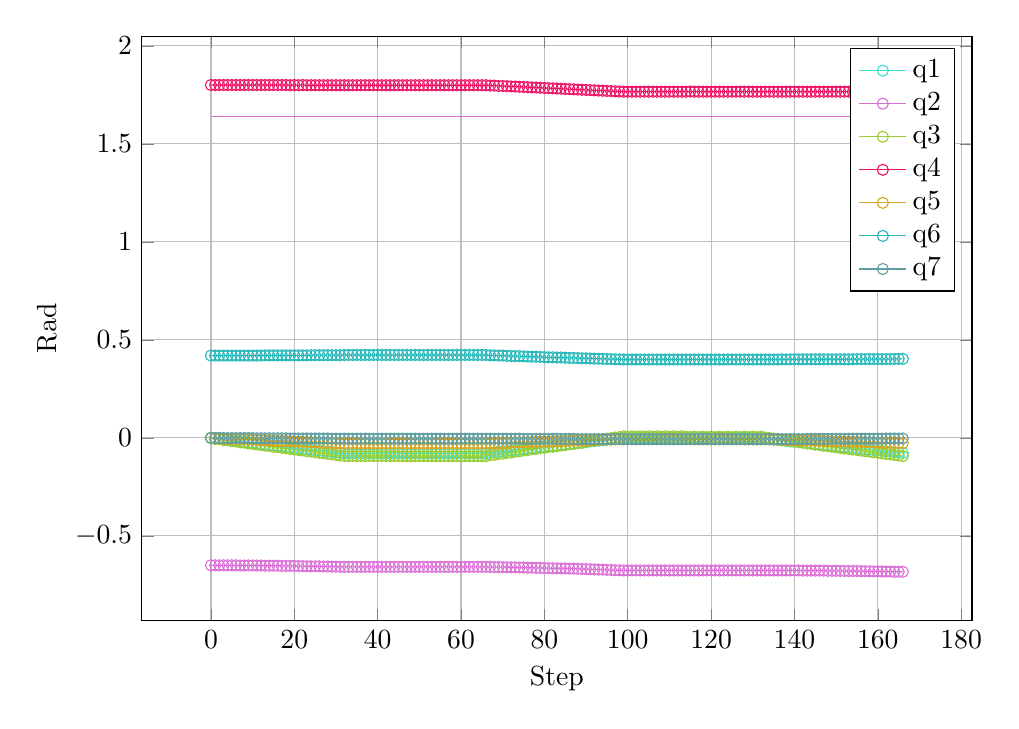
\begin{tikzpicture}
		\begin{axis}[height=9cm, width=\textwidth, grid=major,
		xlabel={Step},ylabel={Rad}
		]
			\addplot [color=Turquoise, mark=o] coordinates {
				(0, 0.000)
				(1, -0.005)
				(2, -0.005)
				(3, -0.010)
				(4, -0.010)
				(5, -0.015)
				(6, -0.015)
				(7, -0.019)
				(8, -0.020)
				(9, -0.024)
				(10, -0.025)
				(11, -0.029)
				(12, -0.030)
				(13, -0.034)
				(14, -0.035)
				(15, -0.039)
				(16, -0.040)
				(17, -0.044)
				(18, -0.045)
				(19, -0.048)
				(20, -0.050)
				(21, -0.053)
				(22, -0.055)
				(23, -0.058)
				(24, -0.060)
				(25, -0.063)
				(26, -0.065)
				(27, -0.067)
				(28, -0.069)
				(29, -0.072)
				(30, -0.074)
				(31, -0.077)
				(32, -0.079)
				(33, -0.080)
				(34, -0.079)
				(35, -0.080)
				(36, -0.079)
				(37, -0.080)
				(38, -0.079)
				(39, -0.080)
				(40, -0.079)
				(41, -0.079)
				(42, -0.079)
				(43, -0.079)
				(44, -0.079)
				(45, -0.079)
				(46, -0.079)
				(47, -0.079)
				(48, -0.079)
				(49, -0.079)
				(50, -0.079)
				(51, -0.079)
				(52, -0.079)
				(53, -0.079)
				(54, -0.079)
				(55, -0.079)
				(56, -0.079)
				(57, -0.079)
				(58, -0.079)
				(59, -0.079)
				(60, -0.079)
				(61, -0.079)
				(62, -0.079)
				(63, -0.079)
				(64, -0.079)
				(65, -0.079)
				(66, -0.079)
				(67, -0.075)
				(68, -0.074)
				(69, -0.070)
				(70, -0.070)
				(71, -0.065)
				(72, -0.065)
				(73, -0.061)
				(74, -0.060)
				(75, -0.056)
				(76, -0.055)
				(77, -0.051)
				(78, -0.050)
				(79, -0.046)
				(80, -0.045)
				(81, -0.042)
				(82, -0.041)
				(83, -0.040)
				(84, -0.036)
				(85, -0.035)
				(86, -0.031)
				(87, -0.030)
				(88, -0.026)
				(89, -0.025)
				(90, -0.022)
				(91, -0.018)
				(92, -0.017)
				(93, -0.014)
				(94, -0.012)
				(95, -0.009)
				(96, -0.008)
				(97, -0.004)
				(98, -0.003)
				(99, 0.000)
				(100, -0.001)
				(101, 0.000)
				(102, -0.001)
				(103, 0.000)
				(104, -0.001)
				(105, 0.000)
				(106, -0.001)
				(107, 0.000)
				(108, -0.001)
				(109, 0.000)
				(110, -0.001)
				(111, 0.000)
				(112, -0.001)
				(113, 0.000)
				(114, -0.001)
				(115, -0.003)
				(116, -0.001)
				(117, -0.003)
				(118, -0.001)
				(119, -0.003)
				(120, -0.001)
				(121, -0.003)
				(122, -0.001)
				(123, -0.003)
				(124, -0.001)
				(125, -0.003)
				(126, -0.001)
				(127, -0.003)
				(128, -0.001)
				(129, -0.003)
				(130, -0.001)
				(131, -0.003)
				(132, -0.001)
				(133, -0.004)
				(134, -0.006)
				(135, -0.009)
				(136, -0.011)
				(137, -0.013)
				(138, -0.015)
				(139, -0.018)
				(140, -0.020)
				(141, -0.022)
				(142, -0.024)
				(143, -0.027)
				(144, -0.029)
				(145, -0.032)
				(146, -0.034)
				(147, -0.036)
				(148, -0.038)
				(149, -0.040)
				(150, -0.043)
				(151, -0.045)
				(152, -0.047)
				(153, -0.049)
				(154, -0.051)
				(155, -0.054)
				(156, -0.056)
				(157, -0.058)
				(158, -0.060)
				(159, -0.062)
				(160, -0.064)
				(161, -0.066)
				(162, -0.069)
				(163, -0.071)
				(164, -0.073)
				(165, -0.075)
				(166, -0.077)
			};
			\addlegendentry{q1}

			\addplot [color=Orchid, mark=o] coordinates {
				(0, -0.650)
				(1, -0.650)
				(2, -0.650)
				(3, -0.650)
				(4, -0.650)
				(5, -0.650)
				(6, -0.650)
				(7, -0.651)
				(8, -0.651)
				(9, -0.651)
				(10, -0.651)
				(11, -0.651)
				(12, -0.651)
				(13, -0.652)
				(14, -0.652)
				(15, -0.652)
				(16, -0.652)
				(17, -0.653)
				(18, -0.653)
				(19, -0.653)
				(20, -0.653)
				(21, -0.654)
				(22, -0.654)
				(23, -0.655)
				(24, -0.655)
				(25, -0.655)
				(26, -0.655)
				(27, -0.656)
				(28, -0.656)
				(29, -0.657)
				(30, -0.657)
				(31, -0.658)
				(32, -0.658)
				(33, -0.658)
				(34, -0.658)
				(35, -0.658)
				(36, -0.658)
				(37, -0.658)
				(38, -0.658)
				(39, -0.658)
				(40, -0.658)
				(41, -0.658)
				(42, -0.658)
				(43, -0.658)
				(44, -0.658)
				(45, -0.658)
				(46, -0.658)
				(47, -0.658)
				(48, -0.658)
				(49, -0.658)
				(50, -0.658)
				(51, -0.658)
				(52, -0.658)
				(53, -0.658)
				(54, -0.658)
				(55, -0.658)
				(56, -0.658)
				(57, -0.658)
				(58, -0.658)
				(59, -0.658)
				(60, -0.658)
				(61, -0.658)
				(62, -0.658)
				(63, -0.658)
				(64, -0.658)
				(65, -0.658)
				(66, -0.658)
				(67, -0.658)
				(68, -0.659)
				(69, -0.659)
				(70, -0.659)
				(71, -0.660)
				(72, -0.660)
				(73, -0.660)
				(74, -0.661)
				(75, -0.661)
				(76, -0.662)
				(77, -0.662)
				(78, -0.663)
				(79, -0.663)
				(80, -0.664)
				(81, -0.664)
				(82, -0.665)
				(83, -0.665)
				(84, -0.666)
				(85, -0.666)
				(86, -0.667)
				(87, -0.667)
				(88, -0.668)
				(89, -0.669)
				(90, -0.669)
				(91, -0.670)
				(92, -0.671)
				(93, -0.672)
				(94, -0.672)
				(95, -0.673)
				(96, -0.674)
				(97, -0.675)
				(98, -0.675)
				(99, -0.676)
				(100, -0.676)
				(101, -0.676)
				(102, -0.676)
				(103, -0.676)
				(104, -0.676)
				(105, -0.676)
				(106, -0.676)
				(107, -0.676)
				(108, -0.676)
				(109, -0.676)
				(110, -0.676)
				(111, -0.676)
				(112, -0.676)
				(113, -0.676)
				(114, -0.676)
				(115, -0.676)
				(116, -0.676)
				(117, -0.676)
				(118, -0.676)
				(119, -0.676)
				(120, -0.676)
				(121, -0.676)
				(122, -0.676)
				(123, -0.676)
				(124, -0.676)
				(125, -0.676)
				(126, -0.676)
				(127, -0.676)
				(128, -0.676)
				(129, -0.676)
				(130, -0.676)
				(131, -0.676)
				(132, -0.676)
				(133, -0.676)
				(134, -0.676)
				(135, -0.676)
				(136, -0.676)
				(137, -0.676)
				(138, -0.676)
				(139, -0.676)
				(140, -0.676)
				(141, -0.676)
				(142, -0.677)
				(143, -0.677)
				(144, -0.677)
				(145, -0.677)
				(146, -0.677)
				(147, -0.677)
				(148, -0.678)
				(149, -0.678)
				(150, -0.678)
				(151, -0.678)
				(152, -0.679)
				(153, -0.679)
				(154, -0.679)
				(155, -0.679)
				(156, -0.680)
				(157, -0.680)
				(158, -0.680)
				(159, -0.681)
				(160, -0.681)
				(161, -0.681)
				(162, -0.682)
				(163, -0.682)
				(164, -0.683)
				(165, -0.683)
				(166, -0.683)
			};
			\addlegendentry{q2}

			\addplot [color=YellowGreen, mark=o] coordinates {
				(0, 0.000)
				(1, -0.006)
				(2, -0.006)
				(3, -0.011)
				(4, -0.012)
				(5, -0.017)
				(6, -0.018)
				(7, -0.023)
				(8, -0.024)
				(9, -0.029)
				(10, -0.030)
				(11, -0.034)
				(12, -0.036)
				(13, -0.040)
				(14, -0.041)
				(15, -0.046)
				(16, -0.047)
				(17, -0.051)
				(18, -0.053)
				(19, -0.057)
				(20, -0.059)
				(21, -0.062)
				(22, -0.064)
				(23, -0.068)
				(24, -0.070)
				(25, -0.073)
				(26, -0.076)
				(27, -0.079)
				(28, -0.081)
				(29, -0.084)
				(30, -0.087)
				(31, -0.090)
				(32, -0.092)
				(33, -0.093)
				(34, -0.092)
				(35, -0.093)
				(36, -0.092)
				(37, -0.093)
				(38, -0.092)
				(39, -0.093)
				(40, -0.092)
				(41, -0.093)
				(42, -0.092)
				(43, -0.093)
				(44, -0.092)
				(45, -0.093)
				(46, -0.093)
				(47, -0.093)
				(48, -0.093)
				(49, -0.093)
				(50, -0.093)
				(51, -0.093)
				(52, -0.093)
				(53, -0.093)
				(54, -0.093)
				(55, -0.093)
				(56, -0.093)
				(57, -0.093)
				(58, -0.093)
				(59, -0.093)
				(60, -0.093)
				(61, -0.093)
				(62, -0.093)
				(63, -0.093)
				(64, -0.093)
				(65, -0.093)
				(66, -0.093)
				(67, -0.087)
				(68, -0.087)
				(69, -0.081)
				(70, -0.081)
				(71, -0.076)
				(72, -0.075)
				(73, -0.070)
				(74, -0.069)
				(75, -0.064)
				(76, -0.063)
				(77, -0.058)
				(78, -0.057)
				(79, -0.052)
				(80, -0.051)
				(81, -0.046)
				(82, -0.045)
				(83, -0.043)
				(84, -0.039)
				(85, -0.037)
				(86, -0.033)
				(87, -0.031)
				(88, -0.027)
				(89, -0.025)
				(90, -0.021)
				(91, -0.016)
				(92, -0.015)
				(93, -0.010)
				(94, -0.008)
				(95, -0.004)
				(96, -0.002)
				(97, 0.002)
				(98, 0.004)
				(99, 0.008)
				(100, 0.006)
				(101, 0.008)
				(102, 0.006)
				(103, 0.008)
				(104, 0.006)
				(105, 0.008)
				(106, 0.006)
				(107, 0.008)
				(108, 0.006)
				(109, 0.008)
				(110, 0.006)
				(111, 0.008)
				(112, 0.006)
				(113, 0.008)
				(114, 0.006)
				(115, 0.004)
				(116, 0.006)
				(117, 0.004)
				(118, 0.006)
				(119, 0.004)
				(120, 0.006)
				(121, 0.004)
				(122, 0.006)
				(123, 0.004)
				(124, 0.006)
				(125, 0.004)
				(126, 0.006)
				(127, 0.004)
				(128, 0.006)
				(129, 0.004)
				(130, 0.006)
				(131, 0.004)
				(132, 0.006)
				(133, 0.002)
				(134, -0.000)
				(135, -0.004)
				(136, -0.006)
				(137, -0.010)
				(138, -0.012)
				(139, -0.016)
				(140, -0.018)
				(141, -0.022)
				(142, -0.024)
				(143, -0.028)
				(144, -0.030)
				(145, -0.034)
				(146, -0.036)
				(147, -0.040)
				(148, -0.042)
				(149, -0.045)
				(150, -0.048)
				(151, -0.051)
				(152, -0.054)
				(153, -0.056)
				(154, -0.059)
				(155, -0.062)
				(156, -0.065)
				(157, -0.068)
				(158, -0.070)
				(159, -0.074)
				(160, -0.076)
				(161, -0.079)
				(162, -0.082)
				(163, -0.084)
				(164, -0.087)
				(165, -0.090)
				(166, -0.093)
			};
			\addlegendentry{q3}

			\addplot [color=WildStrawberry, mark=o] coordinates {
				(0, 1.800)
				(1, 1.800)
				(2, 1.800)
				(3, 1.800)
				(4, 1.800)
				(5, 1.800)
				(6, 1.800)
				(7, 1.800)
				(8, 1.800)
				(9, 1.800)
				(10, 1.800)
				(11, 1.800)
				(12, 1.800)
				(13, 1.800)
				(14, 1.800)
				(15, 1.800)
				(16, 1.800)
				(17, 1.800)
				(18, 1.800)
				(19, 1.799)
				(20, 1.800)
				(21, 1.799)
				(22, 1.800)
				(23, 1.799)
				(24, 1.799)
				(25, 1.799)
				(26, 1.799)
				(27, 1.799)
				(28, 1.799)
				(29, 1.799)
				(30, 1.799)
				(31, 1.799)
				(32, 1.799)
				(33, 1.799)
				(34, 1.799)
				(35, 1.799)
				(36, 1.799)
				(37, 1.799)
				(38, 1.799)
				(39, 1.799)
				(40, 1.799)
				(41, 1.799)
				(42, 1.799)
				(43, 1.799)
				(44, 1.799)
				(45, 1.799)
				(46, 1.799)
				(47, 1.799)
				(48, 1.799)
				(49, 1.799)
				(50, 1.799)
				(51, 1.799)
				(52, 1.799)
				(53, 1.799)
				(54, 1.799)
				(55, 1.799)
				(56, 1.799)
				(57, 1.799)
				(58, 1.799)
				(59, 1.799)
				(60, 1.799)
				(61, 1.799)
				(62, 1.799)
				(63, 1.799)
				(64, 1.799)
				(65, 1.799)
				(66, 1.799)
				(67, 1.797)
				(68, 1.797)
				(69, 1.795)
				(70, 1.795)
				(71, 1.794)
				(72, 1.793)
				(73, 1.792)
				(74, 1.791)
				(75, 1.790)
				(76, 1.789)
				(77, 1.788)
				(78, 1.787)
				(79, 1.786)
				(80, 1.785)
				(81, 1.784)
				(82, 1.783)
				(83, 1.782)
				(84, 1.781)
				(85, 1.780)
				(86, 1.779)
				(87, 1.778)
				(88, 1.777)
				(89, 1.776)
				(90, 1.775)
				(91, 1.774)
				(92, 1.773)
				(93, 1.772)
				(94, 1.771)
				(95, 1.770)
				(96, 1.769)
				(97, 1.768)
				(98, 1.767)
				(99, 1.766)
				(100, 1.766)
				(101, 1.766)
				(102, 1.766)
				(103, 1.766)
				(104, 1.766)
				(105, 1.766)
				(106, 1.766)
				(107, 1.766)
				(108, 1.766)
				(109, 1.766)
				(110, 1.766)
				(111, 1.766)
				(112, 1.766)
				(113, 1.766)
				(114, 1.766)
				(115, 1.767)
				(116, 1.766)
				(117, 1.766)
				(118, 1.766)
				(119, 1.766)
				(120, 1.766)
				(121, 1.766)
				(122, 1.766)
				(123, 1.766)
				(124, 1.766)
				(125, 1.766)
				(126, 1.766)
				(127, 1.766)
				(128, 1.766)
				(129, 1.766)
				(130, 1.766)
				(131, 1.766)
				(132, 1.766)
				(133, 1.766)
				(134, 1.766)
				(135, 1.766)
				(136, 1.766)
				(137, 1.766)
				(138, 1.766)
				(139, 1.766)
				(140, 1.766)
				(141, 1.766)
				(142, 1.766)
				(143, 1.766)
				(144, 1.766)
				(145, 1.766)
				(146, 1.766)
				(147, 1.766)
				(148, 1.766)
				(149, 1.766)
				(150, 1.766)
				(151, 1.766)
				(152, 1.766)
				(153, 1.766)
				(154, 1.766)
				(155, 1.766)
				(156, 1.766)
				(157, 1.766)
				(158, 1.766)
				(159, 1.766)
				(160, 1.766)
				(161, 1.766)
				(162, 1.766)
				(163, 1.766)
				(164, 1.766)
				(165, 1.766)
				(166, 1.766)
			};
			\addlegendentry{q4}

			\addplot [color=Goldenrod, mark=o] coordinates {
				(0, 0.000)
				(1, -0.002)
				(2, -0.002)
				(3, -0.004)
				(4, -0.004)
				(5, -0.005)
				(6, -0.006)
				(7, -0.007)
				(8, -0.007)
				(9, -0.009)
				(10, -0.009)
				(11, -0.011)
				(12, -0.011)
				(13, -0.012)
				(14, -0.013)
				(15, -0.014)
				(16, -0.015)
				(17, -0.016)
				(18, -0.016)
				(19, -0.018)
				(20, -0.018)
				(21, -0.019)
				(22, -0.020)
				(23, -0.021)
				(24, -0.022)
				(25, -0.023)
				(26, -0.023)
				(27, -0.025)
				(28, -0.025)
				(29, -0.026)
				(30, -0.027)
				(31, -0.028)
				(32, -0.029)
				(33, -0.029)
				(34, -0.029)
				(35, -0.029)
				(36, -0.029)
				(37, -0.029)
				(38, -0.029)
				(39, -0.029)
				(40, -0.029)
				(41, -0.029)
				(42, -0.029)
				(43, -0.029)
				(44, -0.029)
				(45, -0.029)
				(46, -0.029)
				(47, -0.029)
				(48, -0.029)
				(49, -0.029)
				(50, -0.029)
				(51, -0.029)
				(52, -0.029)
				(53, -0.029)
				(54, -0.029)
				(55, -0.029)
				(56, -0.029)
				(57, -0.029)
				(58, -0.029)
				(59, -0.029)
				(60, -0.029)
				(61, -0.029)
				(62, -0.029)
				(63, -0.029)
				(64, -0.029)
				(65, -0.029)
				(66, -0.029)
				(67, -0.027)
				(68, -0.027)
				(69, -0.026)
				(70, -0.026)
				(71, -0.025)
				(72, -0.024)
				(73, -0.023)
				(74, -0.023)
				(75, -0.022)
				(76, -0.022)
				(77, -0.020)
				(78, -0.020)
				(79, -0.019)
				(80, -0.019)
				(81, -0.018)
				(82, -0.017)
				(83, -0.017)
				(84, -0.016)
				(85, -0.016)
				(86, -0.015)
				(87, -0.014)
				(88, -0.013)
				(89, -0.013)
				(90, -0.012)
				(91, -0.011)
				(92, -0.011)
				(93, -0.010)
				(94, -0.009)
				(95, -0.009)
				(96, -0.008)
				(97, -0.007)
				(98, -0.007)
				(99, -0.006)
				(100, -0.007)
				(101, -0.006)
				(102, -0.007)
				(103, -0.006)
				(104, -0.006)
				(105, -0.006)
				(106, -0.006)
				(107, -0.006)
				(108, -0.006)
				(109, -0.006)
				(110, -0.006)
				(111, -0.006)
				(112, -0.006)
				(113, -0.006)
				(114, -0.006)
				(115, -0.007)
				(116, -0.006)
				(117, -0.007)
				(118, -0.006)
				(119, -0.007)
				(120, -0.006)
				(121, -0.007)
				(122, -0.006)
				(123, -0.007)
				(124, -0.006)
				(125, -0.007)
				(126, -0.007)
				(127, -0.007)
				(128, -0.007)
				(129, -0.007)
				(130, -0.007)
				(131, -0.007)
				(132, -0.007)
				(133, -0.007)
				(134, -0.008)
				(135, -0.008)
				(136, -0.009)
				(137, -0.010)
				(138, -0.010)
				(139, -0.011)
				(140, -0.012)
				(141, -0.012)
				(142, -0.013)
				(143, -0.013)
				(144, -0.014)
				(145, -0.015)
				(146, -0.015)
				(147, -0.016)
				(148, -0.017)
				(149, -0.017)
				(150, -0.018)
				(151, -0.018)
				(152, -0.019)
				(153, -0.020)
				(154, -0.020)
				(155, -0.021)
				(156, -0.021)
				(157, -0.022)
				(158, -0.022)
				(159, -0.023)
				(160, -0.024)
				(161, -0.024)
				(162, -0.025)
				(163, -0.025)
				(164, -0.026)
				(165, -0.026)
				(166, -0.027)
			};
			\addlegendentry{q5}

			\addplot [color=BlueGreen, mark=o] coordinates {
				(0, 0.420)
				(1, 0.420)
				(2, 0.420)
				(3, 0.420)
				(4, 0.420)
				(5, 0.420)
				(6, 0.420)
				(7, 0.420)
				(8, 0.420)
				(9, 0.420)
				(10, 0.420)
				(11, 0.420)
				(12, 0.420)
				(13, 0.421)
				(14, 0.421)
				(15, 0.421)
				(16, 0.421)
				(17, 0.421)
				(18, 0.421)
				(19, 0.421)
				(20, 0.421)
				(21, 0.421)
				(22, 0.421)
				(23, 0.421)
				(24, 0.422)
				(25, 0.422)
				(26, 0.422)
				(27, 0.422)
				(28, 0.422)
				(29, 0.422)
				(30, 0.422)
				(31, 0.422)
				(32, 0.423)
				(33, 0.423)
				(34, 0.423)
				(35, 0.423)
				(36, 0.423)
				(37, 0.423)
				(38, 0.423)
				(39, 0.423)
				(40, 0.423)
				(41, 0.423)
				(42, 0.423)
				(43, 0.423)
				(44, 0.423)
				(45, 0.423)
				(46, 0.423)
				(47, 0.423)
				(48, 0.423)
				(49, 0.423)
				(50, 0.423)
				(51, 0.423)
				(52, 0.423)
				(53, 0.423)
				(54, 0.423)
				(55, 0.423)
				(56, 0.423)
				(57, 0.423)
				(58, 0.423)
				(59, 0.423)
				(60, 0.423)
				(61, 0.423)
				(62, 0.423)
				(63, 0.423)
				(64, 0.423)
				(65, 0.423)
				(66, 0.423)
				(67, 0.421)
				(68, 0.421)
				(69, 0.420)
				(70, 0.420)
				(71, 0.418)
				(72, 0.418)
				(73, 0.417)
				(74, 0.417)
				(75, 0.416)
				(76, 0.415)
				(77, 0.414)
				(78, 0.414)
				(79, 0.413)
				(80, 0.412)
				(81, 0.411)
				(82, 0.411)
				(83, 0.410)
				(84, 0.410)
				(85, 0.409)
				(86, 0.408)
				(87, 0.408)
				(88, 0.407)
				(89, 0.406)
				(90, 0.406)
				(91, 0.405)
				(92, 0.404)
				(93, 0.404)
				(94, 0.403)
				(95, 0.402)
				(96, 0.402)
				(97, 0.401)
				(98, 0.401)
				(99, 0.400)
				(100, 0.400)
				(101, 0.400)
				(102, 0.400)
				(103, 0.400)
				(104, 0.400)
				(105, 0.400)
				(106, 0.400)
				(107, 0.400)
				(108, 0.400)
				(109, 0.400)
				(110, 0.400)
				(111, 0.400)
				(112, 0.400)
				(113, 0.400)
				(114, 0.400)
				(115, 0.400)
				(116, 0.400)
				(117, 0.400)
				(118, 0.400)
				(119, 0.400)
				(120, 0.400)
				(121, 0.400)
				(122, 0.400)
				(123, 0.400)
				(124, 0.400)
				(125, 0.400)
				(126, 0.400)
				(127, 0.400)
				(128, 0.400)
				(129, 0.400)
				(130, 0.400)
				(131, 0.400)
				(132, 0.400)
				(133, 0.400)
				(134, 0.400)
				(135, 0.400)
				(136, 0.400)
				(137, 0.401)
				(138, 0.400)
				(139, 0.401)
				(140, 0.401)
				(141, 0.401)
				(142, 0.401)
				(143, 0.401)
				(144, 0.401)
				(145, 0.401)
				(146, 0.401)
				(147, 0.401)
				(148, 0.401)
				(149, 0.401)
				(150, 0.401)
				(151, 0.401)
				(152, 0.401)
				(153, 0.401)
				(154, 0.401)
				(155, 0.402)
				(156, 0.402)
				(157, 0.402)
				(158, 0.402)
				(159, 0.402)
				(160, 0.402)
				(161, 0.402)
				(162, 0.402)
				(163, 0.402)
				(164, 0.403)
				(165, 0.403)
				(166, 0.403)
			};
			\addlegendentry{q6}

			\addplot [color=CadetBlue, mark=o] coordinates {
				(0, 0.000)
				(1, -0.000)
				(2, -0.000)
				(3, -0.001)
				(4, -0.001)
				(5, -0.001)
				(6, -0.001)
				(7, -0.001)
				(8, -0.001)
				(9, -0.001)
				(10, -0.001)
				(11, -0.002)
				(12, -0.002)
				(13, -0.002)
				(14, -0.002)
				(15, -0.002)
				(16, -0.002)
				(17, -0.002)
				(18, -0.002)
				(19, -0.003)
				(20, -0.003)
				(21, -0.003)
				(22, -0.003)
				(23, -0.003)
				(24, -0.003)
				(25, -0.003)
				(26, -0.003)
				(27, -0.003)
				(28, -0.003)
				(29, -0.004)
				(30, -0.004)
				(31, -0.004)
				(32, -0.004)
				(33, -0.004)
				(34, -0.004)
				(35, -0.004)
				(36, -0.004)
				(37, -0.004)
				(38, -0.004)
				(39, -0.004)
				(40, -0.004)
				(41, -0.004)
				(42, -0.004)
				(43, -0.004)
				(44, -0.004)
				(45, -0.004)
				(46, -0.004)
				(47, -0.004)
				(48, -0.004)
				(49, -0.004)
				(50, -0.004)
				(51, -0.004)
				(52, -0.004)
				(53, -0.004)
				(54, -0.004)
				(55, -0.004)
				(56, -0.004)
				(57, -0.004)
				(58, -0.004)
				(59, -0.004)
				(60, -0.004)
				(61, -0.004)
				(62, -0.004)
				(63, -0.004)
				(64, -0.004)
				(65, -0.004)
				(66, -0.004)
				(67, -0.004)
				(68, -0.004)
				(69, -0.004)
				(70, -0.004)
				(71, -0.004)
				(72, -0.004)
				(73, -0.004)
				(74, -0.004)
				(75, -0.005)
				(76, -0.005)
				(77, -0.005)
				(78, -0.005)
				(79, -0.005)
				(80, -0.005)
				(81, -0.005)
				(82, -0.005)
				(83, -0.005)
				(84, -0.005)
				(85, -0.005)
				(86, -0.005)
				(87, -0.005)
				(88, -0.006)
				(89, -0.006)
				(90, -0.006)
				(91, -0.006)
				(92, -0.006)
				(93, -0.006)
				(94, -0.006)
				(95, -0.006)
				(96, -0.006)
				(97, -0.006)
				(98, -0.006)
				(99, -0.007)
				(100, -0.007)
				(101, -0.007)
				(102, -0.007)
				(103, -0.007)
				(104, -0.007)
				(105, -0.007)
				(106, -0.007)
				(107, -0.007)
				(108, -0.007)
				(109, -0.007)
				(110, -0.007)
				(111, -0.007)
				(112, -0.007)
				(113, -0.007)
				(114, -0.007)
				(115, -0.006)
				(116, -0.007)
				(117, -0.006)
				(118, -0.007)
				(119, -0.006)
				(120, -0.007)
				(121, -0.006)
				(122, -0.007)
				(123, -0.006)
				(124, -0.007)
				(125, -0.006)
				(126, -0.007)
				(127, -0.006)
				(128, -0.007)
				(129, -0.006)
				(130, -0.007)
				(131, -0.007)
				(132, -0.007)
				(133, -0.006)
				(134, -0.006)
				(135, -0.006)
				(136, -0.006)
				(137, -0.006)
				(138, -0.006)
				(139, -0.006)
				(140, -0.006)
				(141, -0.006)
				(142, -0.006)
				(143, -0.005)
				(144, -0.005)
				(145, -0.005)
				(146, -0.005)
				(147, -0.005)
				(148, -0.005)
				(149, -0.005)
				(150, -0.005)
				(151, -0.005)
				(152, -0.005)
				(153, -0.004)
				(154, -0.004)
				(155, -0.004)
				(156, -0.004)
				(157, -0.004)
				(158, -0.004)
				(159, -0.004)
				(160, -0.004)
				(161, -0.004)
				(162, -0.003)
				(163, -0.003)
				(164, -0.003)
				(165, -0.003)
				(166, -0.003)
			};
			\addlegendentry{q7}

			\addplot[Turquoise,sharp plot,update limits=false] coordinates {				(0,3.14)
				(159,3.14)
			};
			\addplot[Turquoise,sharp plot,update limits=false] coordinates {				(0,-3.14)
				(159,-3.14)
			};

			\addplot[Orchid,sharp plot,update limits=false] coordinates {				(0,1.64)
				(159,1.64)
			};
			\addplot[Orchid,sharp plot,update limits=false] coordinates {				(0,-1.64)
				(159,-1.64)
			};

			\addplot[YellowGreen,sharp plot,update limits=false] coordinates {				(0,3.14)
				(159,3.14)
			};
			\addplot[YellowGreen,sharp plot,update limits=false] coordinates {				(0,-3.14)
				(159,-3.14)
			};

			\addplot[WildStrawberry,sharp plot,update limits=false] coordinates {				(0,2.5)
				(159,2.5)
			};
			\addplot[WildStrawberry,sharp plot,update limits=false] coordinates {				(0,-2.5)
				(159,-2.5)
			};

			\addplot[Goldenrod,sharp plot,update limits=false] coordinates {				(0,4.71)
				(159,4.71)
			};
			\addplot[Goldenrod,sharp plot,update limits=false] coordinates {				(0,-4.71)
				(159,-4.71)
			};

			\addplot[BlueGreen,sharp plot,update limits=false] coordinates {				(0,2.09)
				(159,2.09)
			};
			\addplot[BlueGreen,sharp plot,update limits=false] coordinates {				(0,-2.09)
				(159,-2.09)
			};

			\addplot[CadetBlue,sharp plot,update limits=false] coordinates {				(0,6.28)
				(159,6.28)
			};
			\addplot[CadetBlue,sharp plot,update limits=false] coordinates {
				(0,-6.28)
				(159,-6.28)
			};
		\end{axis}
	\end{tikzpicture}
	\caption{Robot's state while tracking the marker's frame at medium speed.}
	\label{fig:qRobotTrackingMediumPlot}
\end{figure}
}

\providecommand{\cameraPoseTrackingMediumPlot}{
\begin{figure}[!ht]
	\centering
	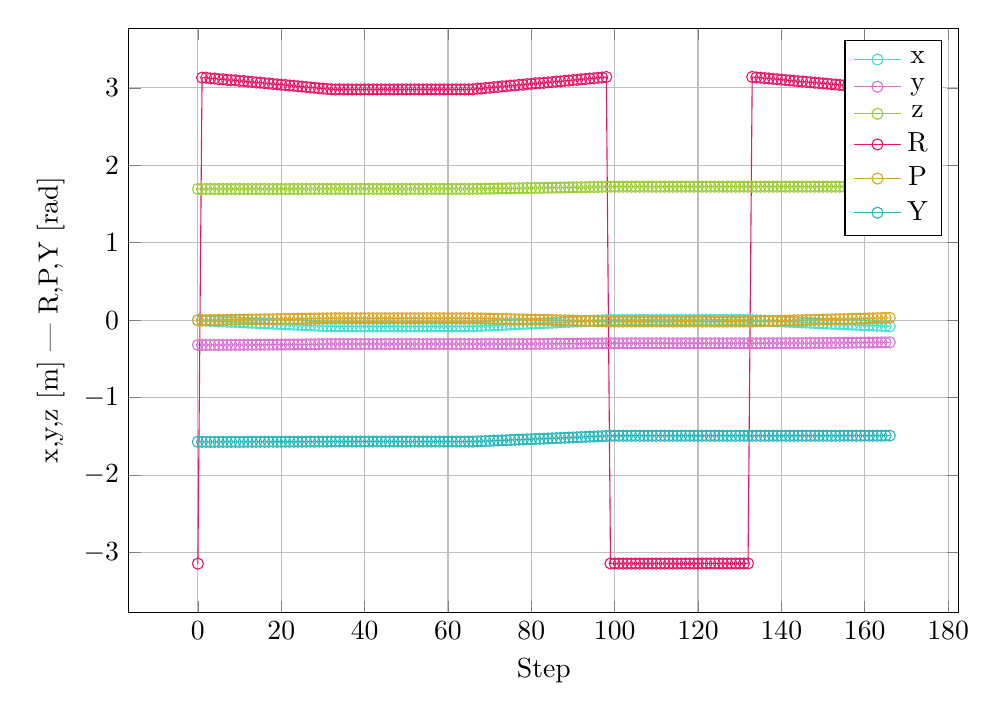
\begin{tikzpicture}
		\begin{axis}[height=9cm, width=\textwidth, grid=major,
		xlabel={Step},ylabel={x,y,z [m] | R,P,Y [rad]}
		]
			\addplot [color=Turquoise, mark=o] coordinates {
				(0, 0.000)
				(1, -0.005)
				(2, -0.005)
				(3, -0.010)
				(4, -0.011)
				(5, -0.015)
				(6, -0.016)
				(7, -0.020)
				(8, -0.021)
				(9, -0.022)
				(10, -0.026)
				(11, -0.027)
				(12, -0.031)
				(13, -0.032)
				(14, -0.036)
				(15, -0.037)
				(16, -0.041)
				(17, -0.042)
				(18, -0.046)
				(19, -0.047)
				(20, -0.051)
				(21, -0.052)
				(22, -0.056)
				(23, -0.057)
				(24, -0.060)
				(25, -0.062)
				(26, -0.065)
				(27, -0.068)
				(28, -0.070)
				(29, -0.073)
				(30, -0.075)
				(31, -0.077)
				(32, -0.079)
				(33, -0.080)
				(34, -0.079)
				(35, -0.080)
				(36, -0.079)
				(37, -0.080)
				(38, -0.080)
				(39, -0.080)
				(40, -0.080)
				(41, -0.080)
				(42, -0.080)
				(43, -0.080)
				(44, -0.080)
				(45, -0.080)
				(46, -0.080)
				(47, -0.080)
				(48, -0.080)
				(49, -0.080)
				(50, -0.080)
				(51, -0.080)
				(52, -0.080)
				(53, -0.080)
				(54, -0.080)
				(55, -0.080)
				(56, -0.080)
				(57, -0.080)
				(58, -0.080)
				(59, -0.080)
				(60, -0.080)
				(61, -0.080)
				(62, -0.080)
				(63, -0.080)
				(64, -0.080)
				(65, -0.080)
				(66, -0.080)
				(67, -0.075)
				(68, -0.075)
				(69, -0.070)
				(70, -0.070)
				(71, -0.065)
				(72, -0.065)
				(73, -0.060)
				(74, -0.059)
				(75, -0.055)
				(76, -0.054)
				(77, -0.050)
				(78, -0.049)
				(79, -0.045)
				(80, -0.044)
				(81, -0.040)
				(82, -0.039)
				(83, -0.038)
				(84, -0.034)
				(85, -0.033)
				(86, -0.029)
				(87, -0.027)
				(88, -0.023)
				(89, -0.022)
				(90, -0.018)
				(91, -0.017)
				(92, -0.013)
				(93, -0.012)
				(94, -0.008)
				(95, -0.007)
				(96, -0.003)
				(97, -0.002)
				(98, 0.002)
				(99, 0.003)
				(100, 0.004)
				(101, 0.003)
				(102, 0.004)
				(103, 0.003)
				(104, 0.004)
				(105, 0.003)
				(106, 0.004)
				(107, 0.004)
				(108, 0.004)
				(109, 0.004)
				(110, 0.004)
				(111, 0.004)
				(112, 0.004)
				(113, 0.004)
				(114, 0.004)
				(115, 0.004)
				(116, 0.004)
				(117, 0.004)
				(118, 0.004)
				(119, 0.004)
				(120, 0.004)
				(121, 0.004)
				(122, 0.004)
				(123, 0.004)
				(124, 0.004)
				(125, 0.004)
				(126, 0.004)
				(127, 0.004)
				(128, 0.004)
				(129, 0.004)
				(130, 0.004)
				(131, 0.004)
				(132, 0.004)
				(133, 0.002)
				(134, -0.001)
				(135, -0.003)
				(136, -0.006)
				(137, -0.008)
				(138, -0.011)
				(139, -0.013)
				(140, -0.016)
				(141, -0.018)
				(142, -0.021)
				(143, -0.023)
				(144, -0.026)
				(145, -0.028)
				(146, -0.031)
				(147, -0.033)
				(148, -0.036)
				(149, -0.038)
				(150, -0.041)
				(151, -0.043)
				(152, -0.046)
				(153, -0.048)
				(154, -0.050)
				(155, -0.052)
				(156, -0.055)
				(157, -0.057)
				(158, -0.060)
				(159, -0.062)
				(160, -0.065)
				(161, -0.067)
				(162, -0.069)
				(163, -0.071)
				(164, -0.074)
				(165, -0.076)
				(166, -0.078)
		};
			\addlegendentry{x}

			\addplot [color=Orchid, mark=o] coordinates {
				(0, -0.319)
				(1, -0.319)
				(2, -0.319)
				(3, -0.319)
				(4, -0.319)
				(5, -0.319)
				(6, -0.319)
				(7, -0.318)
				(8, -0.318)
				(9, -0.318)
				(10, -0.318)
				(11, -0.318)
				(12, -0.317)
				(13, -0.317)
				(14, -0.316)
				(15, -0.316)
				(16, -0.316)
				(17, -0.316)
				(18, -0.315)
				(19, -0.315)
				(20, -0.314)
				(21, -0.314)
				(22, -0.313)
				(23, -0.313)
				(24, -0.312)
				(25, -0.312)
				(26, -0.311)
				(27, -0.310)
				(28, -0.310)
				(29, -0.309)
				(30, -0.308)
				(31, -0.307)
				(32, -0.307)
				(33, -0.307)
				(34, -0.307)
				(35, -0.307)
				(36, -0.307)
				(37, -0.307)
				(38, -0.307)
				(39, -0.307)
				(40, -0.307)
				(41, -0.307)
				(42, -0.307)
				(43, -0.307)
				(44, -0.307)
				(45, -0.307)
				(46, -0.307)
				(47, -0.307)
				(48, -0.307)
				(49, -0.307)
				(50, -0.307)
				(51, -0.307)
				(52, -0.307)
				(53, -0.307)
				(54, -0.307)
				(55, -0.307)
				(56, -0.307)
				(57, -0.307)
				(58, -0.307)
				(59, -0.307)
				(60, -0.307)
				(61, -0.307)
				(62, -0.307)
				(63, -0.307)
				(64, -0.307)
				(65, -0.307)
				(66, -0.307)
				(67, -0.307)
				(68, -0.307)
				(69, -0.307)
				(70, -0.307)
				(71, -0.307)
				(72, -0.307)
				(73, -0.307)
				(74, -0.307)
				(75, -0.307)
				(76, -0.307)
				(77, -0.307)
				(78, -0.306)
				(79, -0.306)
				(80, -0.306)
				(81, -0.306)
				(82, -0.305)
				(83, -0.305)
				(84, -0.305)
				(85, -0.304)
				(86, -0.304)
				(87, -0.304)
				(88, -0.303)
				(89, -0.303)
				(90, -0.302)
				(91, -0.302)
				(92, -0.301)
				(93, -0.301)
				(94, -0.300)
				(95, -0.299)
				(96, -0.299)
				(97, -0.298)
				(98, -0.297)
				(99, -0.297)
				(100, -0.297)
				(101, -0.297)
				(102, -0.297)
				(103, -0.297)
				(104, -0.297)
				(105, -0.297)
				(106, -0.297)
				(107, -0.297)
				(108, -0.297)
				(109, -0.297)
				(110, -0.297)
				(111, -0.297)
				(112, -0.297)
				(113, -0.297)
				(114, -0.297)
				(115, -0.297)
				(116, -0.297)
				(117, -0.297)
				(118, -0.297)
				(119, -0.297)
				(120, -0.297)
				(121, -0.297)
				(122, -0.297)
				(123, -0.297)
				(124, -0.297)
				(125, -0.297)
				(126, -0.297)
				(127, -0.297)
				(128, -0.297)
				(129, -0.297)
				(130, -0.297)
				(131, -0.297)
				(132, -0.297)
				(133, -0.297)
				(134, -0.297)
				(135, -0.297)
				(136, -0.297)
				(137, -0.296)
				(138, -0.296)
				(139, -0.296)
				(140, -0.296)
				(141, -0.296)
				(142, -0.296)
				(143, -0.295)
				(144, -0.295)
				(145, -0.295)
				(146, -0.295)
				(147, -0.294)
				(148, -0.294)
				(149, -0.294)
				(150, -0.293)
				(151, -0.293)
				(152, -0.293)
				(153, -0.292)
				(154, -0.292)
				(155, -0.291)
				(156, -0.291)
				(157, -0.290)
				(158, -0.290)
				(159, -0.289)
				(160, -0.289)
				(161, -0.288)
				(162, -0.288)
				(163, -0.287)
				(164, -0.286)
				(165, -0.286)
				(166, -0.285)
			};
			\addlegendentry{y}

			\addplot [color=YellowGreen, mark=o] coordinates {
				(0, 1.694)
				(1, 1.694)
				(2, 1.694)
				(3, 1.694)
				(4, 1.694)
				(5, 1.694)
				(6, 1.694)
				(7, 1.694)
				(8, 1.694)
				(9, 1.694)
				(10, 1.694)
				(11, 1.694)
				(12, 1.694)
				(13, 1.694)
				(14, 1.694)
				(15, 1.694)
				(16, 1.694)
				(17, 1.694)
				(18, 1.694)
				(19, 1.694)
				(20, 1.694)
				(21, 1.694)
				(22, 1.694)
				(23, 1.694)
				(24, 1.694)
				(25, 1.694)
				(26, 1.695)
				(27, 1.695)
				(28, 1.695)
				(29, 1.695)
				(30, 1.695)
				(31, 1.695)
				(32, 1.695)
				(33, 1.695)
				(34, 1.695)
				(35, 1.695)
				(36, 1.695)
				(37, 1.695)
				(38, 1.695)
				(39, 1.695)
				(40, 1.695)
				(41, 1.695)
				(42, 1.695)
				(43, 1.695)
				(44, 1.695)
				(45, 1.695)
				(46, 1.695)
				(47, 1.695)
				(48, 1.695)
				(49, 1.695)
				(50, 1.695)
				(51, 1.695)
				(52, 1.695)
				(53, 1.695)
				(54, 1.695)
				(55, 1.695)
				(56, 1.695)
				(57, 1.695)
				(58, 1.695)
				(59, 1.695)
				(60, 1.695)
				(61, 1.695)
				(62, 1.695)
				(63, 1.695)
				(64, 1.695)
				(65, 1.695)
				(66, 1.695)
				(67, 1.696)
				(68, 1.696)
				(69, 1.698)
				(70, 1.698)
				(71, 1.700)
				(72, 1.700)
				(73, 1.701)
				(74, 1.702)
				(75, 1.703)
				(76, 1.703)
				(77, 1.705)
				(78, 1.705)
				(79, 1.706)
				(80, 1.707)
				(81, 1.708)
				(82, 1.709)
				(83, 1.709)
				(84, 1.711)
				(85, 1.711)
				(86, 1.712)
				(87, 1.713)
				(88, 1.714)
				(89, 1.715)
				(90, 1.716)
				(91, 1.717)
				(92, 1.718)
				(93, 1.718)
				(94, 1.720)
				(95, 1.720)
				(96, 1.721)
				(97, 1.722)
				(98, 1.723)
				(99, 1.724)
				(100, 1.724)
				(101, 1.724)
				(102, 1.724)
				(103, 1.724)
				(104, 1.724)
				(105, 1.724)
				(106, 1.724)
				(107, 1.724)
				(108, 1.724)
				(109, 1.724)
				(110, 1.724)
				(111, 1.724)
				(112, 1.724)
				(113, 1.724)
				(114, 1.724)
				(115, 1.724)
				(116, 1.724)
				(117, 1.724)
				(118, 1.724)
				(119, 1.724)
				(120, 1.724)
				(121, 1.724)
				(122, 1.724)
				(123, 1.724)
				(124, 1.724)
				(125, 1.724)
				(126, 1.724)
				(127, 1.724)
				(128, 1.724)
				(129, 1.724)
				(130, 1.724)
				(131, 1.724)
				(132, 1.724)
				(133, 1.724)
				(134, 1.724)
				(135, 1.724)
				(136, 1.724)
				(137, 1.724)
				(138, 1.724)
				(139, 1.724)
				(140, 1.724)
				(141, 1.724)
				(142, 1.724)
				(143, 1.724)
				(144, 1.724)
				(145, 1.724)
				(146, 1.724)
				(147, 1.724)
				(148, 1.724)
				(149, 1.724)
				(150, 1.724)
				(151, 1.724)
				(152, 1.724)
				(153, 1.724)
				(154, 1.724)
				(155, 1.724)
				(156, 1.724)
				(157, 1.724)
				(158, 1.724)
				(159, 1.724)
				(160, 1.724)
				(161, 1.724)
				(162, 1.724)
				(163, 1.724)
				(164, 1.724)
				(165, 1.724)
				(166, 1.724)
			};
			\addlegendentry{z}

			\addplot [color=WildStrawberry, mark=o] coordinates {
				(0, -3.142)
				(1, 3.131)
				(2, 3.131)
				(3, 3.121)
				(4, 3.120)
				(5, 3.111)
				(6, 3.110)
				(7, 3.101)
				(8, 3.099)
				(9, 3.098)
				(10, 3.089)
				(11, 3.088)
				(12, 3.079)
				(13, 3.077)
				(14, 3.069)
				(15, 3.067)
				(16, 3.059)
				(17, 3.056)
				(18, 3.049)
				(19, 3.046)
				(20, 3.039)
				(21, 3.036)
				(22, 3.030)
				(23, 3.026)
				(24, 3.020)
				(25, 3.016)
				(26, 3.010)
				(27, 3.004)
				(28, 3.000)
				(29, 2.994)
				(30, 2.990)
				(31, 2.985)
				(32, 2.981)
				(33, 2.978)
				(34, 2.981)
				(35, 2.979)
				(36, 2.980)
				(37, 2.979)
				(38, 2.980)
				(39, 2.979)
				(40, 2.980)
				(41, 2.979)
				(42, 2.980)
				(43, 2.979)
				(44, 2.980)
				(45, 2.979)
				(46, 2.980)
				(47, 2.979)
				(48, 2.980)
				(49, 2.980)
				(50, 2.980)
				(51, 2.980)
				(52, 2.980)
				(53, 2.980)
				(54, 2.980)
				(55, 2.980)
				(56, 2.980)
				(57, 2.980)
				(58, 2.980)
				(59, 2.980)
				(60, 2.980)
				(61, 2.980)
				(62, 2.980)
				(63, 2.980)
				(64, 2.980)
				(65, 2.980)
				(66, 2.980)
				(67, 2.990)
				(68, 2.990)
				(69, 2.999)
				(70, 3.000)
				(71, 3.009)
				(72, 3.010)
				(73, 3.019)
				(74, 3.020)
				(75, 3.029)
				(76, 3.030)
				(77, 3.039)
				(78, 3.040)
				(79, 3.049)
				(80, 3.051)
				(81, 3.059)
				(82, 3.061)
				(83, 3.063)
				(84, 3.071)
				(85, 3.073)
				(86, 3.081)
				(87, 3.083)
				(88, 3.091)
				(89, 3.093)
				(90, 3.101)
				(91, 3.103)
				(92, 3.111)
				(93, 3.113)
				(94, 3.120)
				(95, 3.123)
				(96, 3.130)
				(97, 3.133)
				(98, 3.140)
				(99, -3.140)
				(100, -3.140)
				(101, -3.140)
				(102, -3.140)
				(103, -3.140)
				(104, -3.140)
				(105, -3.140)
				(106, -3.140)
				(107, -3.140)
				(108, -3.140)
				(109, -3.140)
				(110, -3.140)
				(111, -3.140)
				(112, -3.140)
				(113, -3.140)
				(114, -3.140)
				(115, -3.140)
				(116, -3.140)
				(117, -3.140)
				(118, -3.140)
				(119, -3.140)
				(120, -3.140)
				(121, -3.139)
				(122, -3.139)
				(123, -3.139)
				(124, -3.139)
				(125, -3.139)
				(126, -3.139)
				(127, -3.139)
				(128, -3.140)
				(129, -3.139)
				(130, -3.140)
				(131, -3.139)
				(132, -3.139)
				(133, 3.141)
				(134, 3.134)
				(135, 3.131)
				(136, 3.124)
				(137, 3.121)
				(138, 3.115)
				(139, 3.111)
				(140, 3.105)
				(141, 3.101)
				(142, 3.095)
				(143, 3.091)
				(144, 3.085)
				(145, 3.081)
				(146, 3.076)
				(147, 3.072)
				(148, 3.066)
				(149, 3.062)
				(150, 3.056)
				(151, 3.052)
				(152, 3.047)
				(153, 3.043)
				(154, 3.037)
				(155, 3.033)
				(156, 3.028)
				(157, 3.024)
				(158, 3.018)
				(159, 3.014)
				(160, 3.009)
				(161, 3.005)
				(162, 3.000)
				(163, 2.996)
				(164, 2.991)
				(165, 2.987)
				(166, 2.982)
			};
			\addlegendentry{R}

			\addplot [color=Goldenrod, mark=o] coordinates {
				(0, -0.000)
				(1, 0.002)
				(2, 0.002)
				(3, 0.003)
				(4, 0.003)
				(5, 0.005)
				(6, 0.005)
				(7, 0.006)
				(8, 0.007)
				(9, 0.007)
				(10, 0.008)
				(11, 0.008)
				(12, 0.010)
				(13, 0.010)
				(14, 0.011)
				(15, 0.012)
				(16, 0.013)
				(17, 0.013)
				(18, 0.015)
				(19, 0.015)
				(20, 0.016)
				(21, 0.017)
				(22, 0.018)
				(23, 0.018)
				(24, 0.019)
				(25, 0.020)
				(26, 0.021)
				(27, 0.022)
				(28, 0.023)
				(29, 0.024)
				(30, 0.024)
				(31, 0.025)
				(32, 0.026)
				(33, 0.026)
				(34, 0.026)
				(35, 0.026)
				(36, 0.026)
				(37, 0.026)
				(38, 0.026)
				(39, 0.026)
				(40, 0.026)
				(41, 0.026)
				(42, 0.026)
				(43, 0.026)
				(44, 0.026)
				(45, 0.026)
				(46, 0.026)
				(47, 0.026)
				(48, 0.026)
				(49, 0.026)
				(50, 0.026)
				(51, 0.026)
				(52, 0.026)
				(53, 0.026)
				(54, 0.026)
				(55, 0.026)
				(56, 0.026)
				(57, 0.026)
				(58, 0.026)
				(59, 0.026)
				(60, 0.026)
				(61, 0.026)
				(62, 0.026)
				(63, 0.026)
				(64, 0.026)
				(65, 0.026)
				(66, 0.026)
				(67, 0.024)
				(68, 0.024)
				(69, 0.022)
				(70, 0.021)
				(71, 0.019)
				(72, 0.019)
				(73, 0.017)
				(74, 0.017)
				(75, 0.014)
				(76, 0.014)
				(77, 0.012)
				(78, 0.012)
				(79, 0.009)
				(80, 0.009)
				(81, 0.007)
				(82, 0.006)
				(83, 0.006)
				(84, 0.004)
				(85, 0.003)
				(86, 0.001)
				(87, 0.000)
				(88, -0.002)
				(89, -0.002)
				(90, -0.004)
				(91, -0.005)
				(92, -0.007)
				(93, -0.008)
				(94, -0.010)
				(95, -0.011)
				(96, -0.013)
				(97, -0.013)
				(98, -0.015)
				(99, -0.016)
				(100, -0.016)
				(101, -0.016)
				(102, -0.016)
				(103, -0.016)
				(104, -0.016)
				(105, -0.016)
				(106, -0.016)
				(107, -0.016)
				(108, -0.016)
				(109, -0.016)
				(110, -0.016)
				(111, -0.016)
				(112, -0.016)
				(113, -0.016)
				(114, -0.016)
				(115, -0.016)
				(116, -0.016)
				(117, -0.016)
				(118, -0.016)
				(119, -0.016)
				(120, -0.016)
				(121, -0.017)
				(122, -0.017)
				(123, -0.017)
				(124, -0.017)
				(125, -0.017)
				(126, -0.017)
				(127, -0.017)
				(128, -0.016)
				(129, -0.017)
				(130, -0.016)
				(131, -0.017)
				(132, -0.017)
				(133, -0.016)
				(134, -0.014)
				(135, -0.013)
				(136, -0.011)
				(137, -0.010)
				(138, -0.008)
				(139, -0.007)
				(140, -0.005)
				(141, -0.004)
				(142, -0.002)
				(143, -0.001)
				(144, 0.000)
				(145, 0.001)
				(146, 0.003)
				(147, 0.004)
				(148, 0.006)
				(149, 0.007)
				(150, 0.009)
				(151, 0.010)
				(152, 0.012)
				(153, 0.013)
				(154, 0.014)
				(155, 0.016)
				(156, 0.017)
				(157, 0.018)
				(158, 0.020)
				(159, 0.021)
				(160, 0.023)
				(161, 0.024)
				(162, 0.026)
				(163, 0.027)
				(164, 0.029)
				(165, 0.030)
				(166, 0.031)
			};
			\addlegendentry{P}

			\addplot [color=BlueGreen, mark=o] coordinates {
				(0, -1.570)
				(1, -1.570)
				(2, -1.570)
				(3, -1.570)
				(4, -1.570)
				(5, -1.570)
				(6, -1.570)
				(7, -1.570)
				(8, -1.570)
				(9, -1.570)
				(10, -1.570)
				(11, -1.570)
				(12, -1.569)
				(13, -1.569)
				(14, -1.569)
				(15, -1.569)
				(16, -1.569)
				(17, -1.569)
				(18, -1.568)
				(19, -1.569)
				(20, -1.568)
				(21, -1.568)
				(22, -1.568)
				(23, -1.568)
				(24, -1.567)
				(25, -1.568)
				(26, -1.567)
				(27, -1.566)
				(28, -1.567)
				(29, -1.566)
				(30, -1.566)
				(31, -1.566)
				(32, -1.566)
				(33, -1.565)
				(34, -1.566)
				(35, -1.565)
				(36, -1.566)
				(37, -1.565)
				(38, -1.566)
				(39, -1.565)
				(40, -1.566)
				(41, -1.565)
				(42, -1.566)
				(43, -1.565)
				(44, -1.566)
				(45, -1.565)
				(46, -1.566)
				(47, -1.565)
				(48, -1.566)
				(49, -1.566)
				(50, -1.566)
				(51, -1.566)
				(52, -1.566)
				(53, -1.566)
				(54, -1.566)
				(55, -1.566)
				(56, -1.566)
				(57, -1.566)
				(58, -1.566)
				(59, -1.566)
				(60, -1.566)
				(61, -1.566)
				(62, -1.566)
				(63, -1.566)
				(64, -1.566)
				(65, -1.566)
				(66, -1.567)
				(67, -1.562)
				(68, -1.562)
				(69, -1.558)
				(70, -1.558)
				(71, -1.554)
				(72, -1.553)
				(73, -1.550)
				(74, -1.549)
				(75, -1.545)
				(76, -1.544)
				(77, -1.541)
				(78, -1.540)
				(79, -1.536)
				(80, -1.535)
				(81, -1.532)
				(82, -1.531)
				(83, -1.529)
				(84, -1.526)
				(85, -1.524)
				(86, -1.521)
				(87, -1.520)
				(88, -1.517)
				(89, -1.515)
				(90, -1.512)
				(91, -1.510)
				(92, -1.507)
				(93, -1.505)
				(94, -1.502)
				(95, -1.501)
				(96, -1.498)
				(97, -1.496)
				(98, -1.493)
				(99, -1.491)
				(100, -1.491)
				(101, -1.491)
				(102, -1.491)
				(103, -1.491)
				(104, -1.491)
				(105, -1.491)
				(106, -1.491)
				(107, -1.491)
				(108, -1.491)
				(109, -1.491)
				(110, -1.491)
				(111, -1.491)
				(112, -1.491)
				(113, -1.491)
				(114, -1.491)
				(115, -1.491)
				(116, -1.491)
				(117, -1.491)
				(118, -1.491)
				(119, -1.491)
				(120, -1.491)
				(121, -1.491)
				(122, -1.491)
				(123, -1.491)
				(124, -1.491)
				(125, -1.491)
				(126, -1.491)
				(127, -1.491)
				(128, -1.491)
				(129, -1.491)
				(130, -1.491)
				(131, -1.491)
				(132, -1.491)
				(133, -1.491)
				(134, -1.491)
				(135, -1.491)
				(136, -1.491)
				(137, -1.491)
				(138, -1.491)
				(139, -1.491)
				(140, -1.491)
				(141, -1.491)
				(142, -1.491)
				(143, -1.491)
				(144, -1.491)
				(145, -1.491)
				(146, -1.491)
				(147, -1.491)
				(148, -1.491)
				(149, -1.491)
				(150, -1.491)
				(151, -1.491)
				(152, -1.491)
				(153, -1.491)
				(154, -1.491)
				(155, -1.490)
				(156, -1.490)
				(157, -1.490)
				(158, -1.490)
				(159, -1.490)
				(160, -1.490)
				(161, -1.490)
				(162, -1.490)
				(163, -1.490)
				(164, -1.490)
				(165, -1.489)
				(166, -1.489)
			};
			\addlegendentry{Y}

		\end{axis}
	\end{tikzpicture}
	\caption{Robot camera's frame while tracking the marker's frame at medium speed.}
	\label{fig:cameraPoseTrackingMediumPlot}
\end{figure}
}

\providecommand{\speedTrackingMediumPlot}{
\begin{figure}[!ht]
	\centering
	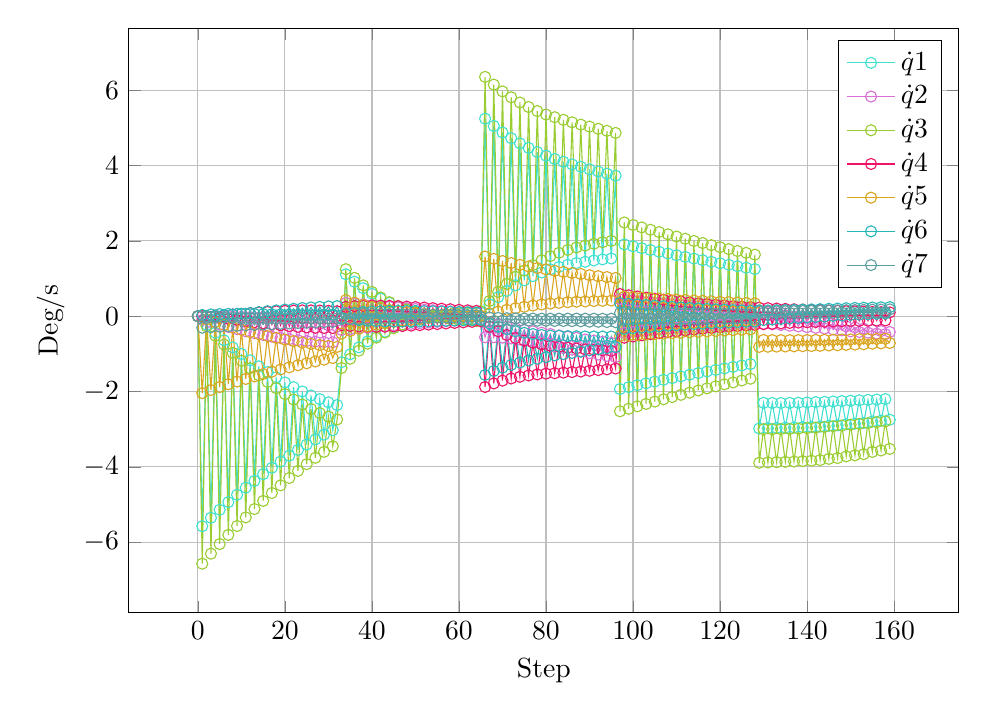
\begin{tikzpicture}
		\begin{axis}[height=9cm, width=\textwidth, grid=major,
		xlabel={Step},ylabel={Deg/s}
		]
			\addplot [color=Turquoise, mark=o] coordinates {
				(0, 0.000)
				(1, -5.577)
				(2, -0.227)
				(3, -5.354)
				(4, -0.439)
				(5, -5.141)
				(6, -0.638)
				(7, -4.938)
				(8, -0.826)
				(9, -4.742)
				(10, -1.003)
				(11, -4.554)
				(12, -1.171)
				(13, -4.372)
				(14, -1.331)
				(15, -4.196)
				(16, -1.482)
				(17, -4.026)
				(18, -1.624)
				(19, -3.862)
				(20, -1.759)
				(21, -3.704)
				(22, -1.884)
				(23, -3.552)
				(24, -2.000)
				(25, -3.408)
				(26, -2.106)
				(27, -3.272)
				(28, -2.202)
				(29, -3.145)
				(30, -2.287)
				(31, -3.028)
				(32, -2.359)
				(33, -1.222)
				(34, 1.114)
				(35, -1.011)
				(36, 0.916)
				(37, -0.827)
				(38, 0.744)
				(39, -0.667)
				(40, 0.596)
				(41, -0.529)
				(42, 0.468)
				(43, -0.411)
				(44, 0.358)
				(45, -0.310)
				(46, 0.266)
				(47, -0.225)
				(48, 0.187)
				(49, -0.153)
				(50, 0.122)
				(51, -0.093)
				(52, 0.068)
				(53, -0.044)
				(54, 0.023)
				(55, -0.004)
				(56, -0.012)
				(57, 0.027)
				(58, -0.041)
				(59, 0.053)
				(60, -0.063)
				(61, 0.072)
				(62, -0.080)
				(63, 0.086)
				(64, -0.092)
				(65, 0.096)
				(66, 5.249)
				(67, 0.313)
				(68, 5.055)
				(69, 0.506)
				(70, 4.882)
				(71, 0.675)
				(72, 4.729)
				(73, 0.823)
				(74, 4.592)
				(75, 0.953)
				(76, 4.471)
				(77, 1.065)
				(78, 4.362)
				(79, 1.162)
				(80, 4.265)
				(81, 1.246)
				(82, 4.178)
				(83, 1.310)
				(84, 4.103)
				(85, 1.366)
				(86, 4.034)
				(87, 1.414)
				(88, 3.969)
				(89, 1.447)
				(90, 3.903)
				(91, 1.481)
				(92, 3.845)
				(93, 1.510)
				(94, 3.788)
				(95, 1.534)
				(96, 3.733)
				(97, -1.934)
				(98, 1.908)
				(99, -1.883)
				(100, 1.857)
				(101, -1.832)
				(102, 1.808)
				(103, -1.783)
				(104, 1.759)
				(105, -1.736)
				(106, 1.712)
				(107, -1.689)
				(108, 1.666)
				(109, -1.644)
				(110, 1.621)
				(111, -1.599)
				(112, 1.577)
				(113, -1.554)
				(114, 1.532)
				(115, -1.510)
				(116, 1.489)
				(117, -1.468)
				(118, 1.447)
				(119, -1.426)
				(120, 1.406)
				(121, -1.386)
				(122, 1.366)
				(123, -1.346)
				(124, 1.327)
				(125, -1.308)
				(126, 1.289)
				(127, -1.271)
				(128, 1.253)
				(129, -2.982)
				(130, -2.300)
				(131, -2.974)
				(132, -2.304)
				(133, -2.967)
				(134, -2.304)
				(135, -2.960)
				(136, -2.302)
				(137, -2.954)
				(138, -2.298)
				(139, -2.947)
				(140, -2.291)
				(141, -2.940)
				(142, -2.283)
				(143, -2.932)
				(144, -2.274)
				(145, -2.910)
				(146, -2.265)
				(147, -2.899)
				(148, -2.254)
				(149, -2.870)
				(150, -2.244)
				(151, -2.854)
				(152, -2.233)
				(153, -2.836)
				(154, -2.222)
				(155, -2.797)
				(156, -2.213)
				(157, -2.774)
				(158, -2.202)
				(159, -2.749)
			};
			\addlegendentry{$\dot q$1}

			\addplot [color=Orchid, mark=o] coordinates {
				(0, 0.000)
				(1, -0.095)
				(2, -0.001)
				(3, -0.159)
				(4, -0.002)
				(5, -0.223)
				(6, -0.005)
				(7, -0.284)
				(8, -0.008)
				(9, -0.343)
				(10, -0.014)
				(11, -0.399)
				(12, -0.023)
				(13, -0.451)
				(14, -0.034)
				(15, -0.499)
				(16, -0.048)
				(17, -0.542)
				(18, -0.066)
				(19, -0.579)
				(20, -0.087)
				(21, -0.611)
				(22, -0.112)
				(23, -0.638)
				(24, -0.140)
				(25, -0.659)
				(26, -0.171)
				(27, -0.675)
				(28, -0.205)
				(29, -0.686)
				(30, -0.241)
				(31, -0.693)
				(32, -0.278)
				(33, -0.364)
				(34, 0.355)
				(35, -0.347)
				(36, 0.337)
				(37, -0.327)
				(38, 0.317)
				(39, -0.307)
				(40, 0.296)
				(41, -0.286)
				(42, 0.275)
				(43, -0.265)
				(44, 0.254)
				(45, -0.244)
				(46, 0.233)
				(47, -0.223)
				(48, 0.213)
				(49, -0.203)
				(50, 0.194)
				(51, -0.185)
				(52, 0.175)
				(53, -0.167)
				(54, 0.158)
				(55, -0.150)
				(56, 0.142)
				(57, -0.134)
				(58, 0.126)
				(59, -0.119)
				(60, 0.112)
				(61, -0.106)
				(62, 0.099)
				(63, -0.093)
				(64, 0.087)
				(65, -0.082)
				(66, -0.558)
				(67, -0.155)
				(68, -0.558)
				(69, -0.217)
				(70, -0.569)
				(71, -0.271)
				(72, -0.589)
				(73, -0.319)
				(74, -0.616)
				(75, -0.361)
				(76, -0.648)
				(77, -0.400)
				(78, -0.684)
				(79, -0.437)
				(80, -0.723)
				(81, -0.471)
				(82, -0.805)
				(83, -0.512)
				(84, -0.846)
				(85, -0.543)
				(86, -0.888)
				(87, -0.574)
				(88, -0.929)
				(89, -0.617)
				(90, -0.981)
				(91, -0.647)
				(92, -1.018)
				(93, -0.677)
				(94, -1.053)
				(95, -0.708)
				(96, -1.086)
				(97, 0.452)
				(98, -0.445)
				(99, 0.426)
				(100, -0.419)
				(101, 0.401)
				(102, -0.394)
				(103, 0.378)
				(104, -0.371)
				(105, 0.355)
				(106, -0.350)
				(107, 0.335)
				(108, -0.329)
				(109, 0.315)
				(110, -0.310)
				(111, 0.297)
				(112, -0.295)
				(113, 0.282)
				(114, -0.278)
				(115, 0.265)
				(116, -0.261)
				(117, 0.249)
				(118, -0.245)
				(119, 0.234)
				(120, -0.230)
				(121, 0.220)
				(122, -0.216)
				(123, 0.207)
				(124, -0.203)
				(125, 0.194)
				(126, -0.191)
				(127, 0.182)
				(128, -0.179)
				(129, 0.156)
				(130, -0.199)
				(131, 0.112)
				(132, -0.216)
				(133, 0.069)
				(134, -0.234)
				(135, 0.027)
				(136, -0.252)
				(137, -0.014)
				(138, -0.270)
				(139, -0.054)
				(140, -0.289)
				(141, -0.092)
				(142, -0.308)
				(143, -0.130)
				(144, -0.327)
				(145, -0.185)
				(146, -0.355)
				(147, -0.219)
				(148, -0.374)
				(149, -0.269)
				(150, -0.402)
				(151, -0.299)
				(152, -0.419)
				(153, -0.328)
				(154, -0.436)
				(155, -0.370)
				(156, -0.461)
				(157, -0.395)
				(158, -0.477)
				(159, -0.418)
			};
			\addlegendentry{$\dot q$2}

			\addplot [color=YellowGreen, mark=o] coordinates {
				(0, 0.000)
				(1, -6.574)
				(2, -0.268)
				(3, -6.307)
				(4, -0.518)
				(5, -6.053)
				(6, -0.752)
				(7, -5.809)
				(8, -0.974)
				(9, -5.573)
				(10, -1.183)
				(11, -5.344)
				(12, -1.381)
				(13, -5.122)
				(14, -1.568)
				(15, -4.906)
				(16, -1.745)
				(17, -4.696)
				(18, -1.912)
				(19, -4.493)
				(20, -2.068)
				(21, -4.297)
				(22, -2.213)
				(23, -4.109)
				(24, -2.346)
				(25, -3.930)
				(26, -2.467)
				(27, -3.761)
				(28, -2.573)
				(29, -3.603)
				(30, -2.666)
				(31, -3.456)
				(32, -2.743)
				(33, -1.376)
				(34, 1.249)
				(35, -1.129)
				(36, 1.019)
				(37, -0.915)
				(38, 0.819)
				(39, -0.729)
				(40, 0.647)
				(41, -0.570)
				(42, 0.499)
				(43, -0.434)
				(44, 0.374)
				(45, -0.318)
				(46, 0.268)
				(47, -0.221)
				(48, 0.179)
				(49, -0.140)
				(50, 0.105)
				(51, -0.073)
				(52, 0.045)
				(53, -0.019)
				(54, -0.004)
				(55, 0.025)
				(56, -0.044)
				(57, 0.060)
				(58, -0.074)
				(59, 0.087)
				(60, -0.097)
				(61, 0.107)
				(62, -0.115)
				(63, 0.121)
				(64, -0.127)
				(65, 0.131)
				(66, 6.358)
				(67, 0.404)
				(68, 6.153)
				(69, 0.646)
				(70, 5.973)
				(71, 0.860)
				(72, 5.816)
				(73, 1.049)
				(74, 5.678)
				(75, 1.215)
				(76, 5.558)
				(77, 1.360)
				(78, 5.451)
				(79, 1.487)
				(80, 5.358)
				(81, 1.597)
				(82, 5.287)
				(83, 1.685)
				(84, 5.217)
				(85, 1.761)
				(86, 5.151)
				(87, 1.827)
				(88, 5.090)
				(89, 1.877)
				(90, 5.037)
				(91, 1.925)
				(92, 4.980)
				(93, 1.965)
				(94, 4.925)
				(95, 2.001)
				(96, 4.870)
				(97, -2.526)
				(98, 2.491)
				(99, -2.459)
				(100, 2.425)
				(101, -2.393)
				(102, 2.360)
				(103, -2.329)
				(104, 2.297)
				(105, -2.267)
				(106, 2.236)
				(107, -2.206)
				(108, 2.176)
				(109, -2.147)
				(110, 2.117)
				(111, -2.089)
				(112, 2.058)
				(113, -2.030)
				(114, 2.000)
				(115, -1.972)
				(116, 1.944)
				(117, -1.916)
				(118, 1.889)
				(119, -1.862)
				(120, 1.835)
				(121, -1.809)
				(122, 1.783)
				(123, -1.758)
				(124, 1.732)
				(125, -1.708)
				(126, 1.683)
				(127, -1.660)
				(128, 1.636)
				(129, -3.894)
				(130, -3.002)
				(131, -3.885)
				(132, -3.004)
				(133, -3.877)
				(134, -3.001)
				(135, -3.868)
				(136, -2.995)
				(137, -3.859)
				(138, -2.986)
				(139, -3.849)
				(140, -2.973)
				(141, -3.837)
				(142, -2.959)
				(143, -3.822)
				(144, -2.942)
				(145, -3.789)
				(146, -2.922)
				(147, -3.768)
				(148, -2.903)
				(149, -3.723)
				(150, -2.881)
				(151, -3.696)
				(152, -2.860)
				(153, -3.665)
				(154, -2.839)
				(155, -3.604)
				(156, -2.816)
				(157, -3.566)
				(158, -2.795)
				(159, -3.525)
			};
			\addlegendentry{$\dot q$3}

			\addplot [color=WildStrawberry, mark=o] coordinates {
				(0, 0.000)
				(1, 0.002)
				(2, 0.004)
				(3, -0.018)
				(4, 0.014)
				(5, -0.042)
				(6, 0.028)
				(7, -0.069)
				(8, 0.045)
				(9, -0.099)
				(10, 0.063)
				(11, -0.129)
				(12, 0.081)
				(13, -0.160)
				(14, 0.100)
				(15, -0.189)
				(16, 0.116)
				(17, -0.217)
				(18, 0.131)
				(19, -0.242)
				(20, 0.142)
				(21, -0.264)
				(22, 0.150)
				(23, -0.283)
				(24, 0.155)
				(25, -0.297)
				(26, 0.155)
				(27, -0.307)
				(28, 0.151)
				(29, -0.313)
				(30, 0.142)
				(31, -0.314)
				(32, 0.131)
				(33, -0.237)
				(34, 0.250)
				(35, -0.259)
				(36, 0.268)
				(37, -0.273)
				(38, 0.278)
				(39, -0.280)
				(40, 0.282)
				(41, -0.282)
				(42, 0.281)
				(43, -0.278)
				(44, 0.275)
				(45, -0.271)
				(46, 0.267)
				(47, -0.262)
				(48, 0.256)
				(49, -0.250)
				(50, 0.243)
				(51, -0.237)
				(52, 0.230)
				(53, -0.222)
				(54, 0.215)
				(55, -0.208)
				(56, 0.200)
				(57, -0.193)
				(58, 0.185)
				(59, -0.178)
				(60, 0.170)
				(61, -0.163)
				(62, 0.156)
				(63, -0.149)
				(64, 0.142)
				(65, -0.135)
				(66, -1.880)
				(67, -0.280)
				(68, -1.785)
				(69, -0.400)
				(70, -1.711)
				(71, -0.499)
				(72, -1.653)
				(73, -0.580)
				(74, -1.608)
				(75, -0.647)
				(76, -1.573)
				(77, -0.703)
				(78, -1.546)
				(79, -0.748)
				(80, -1.524)
				(81, -0.786)
				(82, -1.514)
				(83, -0.811)
				(84, -1.498)
				(85, -0.835)
				(86, -1.484)
				(87, -0.855)
				(88, -1.469)
				(89, -0.880)
				(90, -1.449)
				(91, -0.894)
				(92, -1.431)
				(93, -0.906)
				(94, -1.411)
				(95, -0.918)
				(96, -1.389)
				(97, 0.590)
				(98, -0.571)
				(99, 0.556)
				(100, -0.538)
				(101, 0.524)
				(102, -0.507)
				(103, 0.494)
				(104, -0.478)
				(105, 0.466)
				(106, -0.451)
				(107, 0.439)
				(108, -0.425)
				(109, 0.414)
				(110, -0.400)
				(111, 0.390)
				(112, -0.375)
				(113, 0.365)
				(114, -0.353)
				(115, 0.343)
				(116, -0.331)
				(117, 0.323)
				(118, -0.312)
				(119, 0.303)
				(120, -0.293)
				(121, 0.285)
				(122, -0.275)
				(123, 0.268)
				(124, -0.259)
				(125, 0.252)
				(126, -0.243)
				(127, 0.237)
				(128, -0.229)
				(129, 0.227)
				(130, -0.212)
				(131, 0.215)
				(132, -0.200)
				(133, 0.204)
				(134, -0.189)
				(135, 0.194)
				(136, -0.178)
				(137, 0.184)
				(138, -0.169)
				(139, 0.176)
				(140, -0.161)
				(141, 0.168)
				(142, -0.154)
				(143, 0.160)
				(144, -0.147)
				(145, 0.150)
				(146, -0.138)
				(147, 0.144)
				(148, -0.133)
				(149, 0.134)
				(150, -0.126)
				(151, 0.129)
				(152, -0.123)
				(153, 0.123)
				(154, -0.120)
				(155, 0.114)
				(156, -0.115)
				(157, 0.108)
				(158, -0.113)
				(159, 0.102)
			};
			\addlegendentry{$\dot q$4}

			\addplot [color=Goldenrod, mark=o] coordinates {
				(0, 0.000)
				(1, -2.042)
				(2, -0.083)
				(3, -1.960)
				(4, -0.160)
				(5, -1.881)
				(6, -0.232)
				(7, -1.806)
				(8, -0.300)
				(9, -1.735)
				(10, -0.363)
				(11, -1.666)
				(12, -0.422)
				(13, -1.599)
				(14, -0.477)
				(15, -1.535)
				(16, -0.528)
				(17, -1.473)
				(18, -0.576)
				(19, -1.414)
				(20, -0.621)
				(21, -1.357)
				(22, -0.662)
				(23, -1.302)
				(24, -0.700)
				(25, -1.250)
				(26, -0.734)
				(27, -1.201)
				(28, -0.765)
				(29, -1.154)
				(30, -0.791)
				(31, -1.111)
				(32, -0.814)
				(33, -0.463)
				(34, 0.427)
				(35, -0.392)
				(36, 0.360)
				(37, -0.329)
				(38, 0.301)
				(39, -0.274)
				(40, 0.249)
				(41, -0.225)
				(42, 0.204)
				(43, -0.183)
				(44, 0.164)
				(45, -0.147)
				(46, 0.130)
				(47, -0.115)
				(48, 0.101)
				(49, -0.088)
				(50, 0.076)
				(51, -0.065)
				(52, 0.055)
				(53, -0.046)
				(54, 0.038)
				(55, -0.030)
				(56, 0.023)
				(57, -0.017)
				(58, 0.011)
				(59, -0.006)
				(60, 0.001)
				(61, 0.003)
				(62, -0.007)
				(63, 0.010)
				(64, -0.013)
				(65, 0.015)
				(66, 1.585)
				(67, 0.073)
				(68, 1.523)
				(69, 0.125)
				(70, 1.466)
				(71, 0.172)
				(72, 1.413)
				(73, 0.214)
				(74, 1.365)
				(75, 0.251)
				(76, 1.321)
				(77, 0.284)
				(78, 1.280)
				(79, 0.312)
				(80, 1.244)
				(81, 0.336)
				(82, 1.207)
				(83, 0.356)
				(84, 1.177)
				(85, 0.372)
				(86, 1.149)
				(87, 0.386)
				(88, 1.122)
				(89, 0.393)
				(90, 1.090)
				(91, 0.402)
				(92, 1.065)
				(93, 0.410)
				(94, 1.041)
				(95, 0.416)
				(96, 1.016)
				(97, -0.527)
				(98, 0.520)
				(99, -0.513)
				(100, 0.506)
				(101, -0.500)
				(102, 0.493)
				(103, -0.487)
				(104, 0.480)
				(105, -0.474)
				(106, 0.467)
				(107, -0.461)
				(108, 0.455)
				(109, -0.449)
				(110, 0.442)
				(111, -0.437)
				(112, 0.430)
				(113, -0.424)
				(114, 0.418)
				(115, -0.412)
				(116, 0.406)
				(117, -0.401)
				(118, 0.395)
				(119, -0.389)
				(120, 0.384)
				(121, -0.378)
				(122, 0.373)
				(123, -0.368)
				(124, 0.362)
				(125, -0.357)
				(126, 0.352)
				(127, -0.347)
				(128, 0.342)
				(129, -0.815)
				(130, -0.631)
				(131, -0.811)
				(132, -0.634)
				(133, -0.807)
				(134, -0.635)
				(135, -0.804)
				(136, -0.635)
				(137, -0.800)
				(138, -0.634)
				(139, -0.796)
				(140, -0.632)
				(141, -0.791)
				(142, -0.629)
				(143, -0.786)
				(144, -0.626)
				(145, -0.777)
				(146, -0.623)
				(147, -0.771)
				(148, -0.619)
				(149, -0.760)
				(150, -0.615)
				(151, -0.753)
				(152, -0.610)
				(153, -0.745)
				(154, -0.606)
				(155, -0.730)
				(156, -0.601)
				(157, -0.721)
				(158, -0.597)
				(159, -0.711)
			};
			\addlegendentry{$\dot q$5}

			\addplot [color=BlueGreen, mark=o] coordinates {
				(0, 0.000)
				(1, 0.034)
				(2, 0.004)
				(3, 0.048)
				(4, 0.014)
				(5, 0.057)
				(6, 0.028)
				(7, 0.062)
				(8, 0.045)
				(9, 0.064)
				(10, 0.065)
				(11, 0.063)
				(12, 0.087)
				(13, 0.060)
				(14, 0.109)
				(15, 0.057)
				(16, 0.133)
				(17, 0.052)
				(18, 0.155)
				(19, 0.048)
				(20, 0.178)
				(21, 0.043)
				(22, 0.198)
				(23, 0.040)
				(24, 0.217)
				(25, 0.038)
				(26, 0.234)
				(27, 0.038)
				(28, 0.248)
				(29, 0.039)
				(30, 0.260)
				(31, 0.042)
				(32, 0.269)
				(33, -0.047)
				(34, 0.064)
				(35, -0.078)
				(36, 0.091)
				(37, -0.102)
				(38, 0.112)
				(39, -0.119)
				(40, 0.126)
				(41, -0.131)
				(42, 0.135)
				(43, -0.139)
				(44, 0.141)
				(45, -0.142)
				(46, 0.143)
				(47, -0.143)
				(48, 0.143)
				(49, -0.142)
				(50, 0.141)
				(51, -0.139)
				(52, 0.136)
				(53, -0.134)
				(54, 0.131)
				(55, -0.128)
				(56, 0.125)
				(57, -0.121)
				(58, 0.118)
				(59, -0.114)
				(60, 0.110)
				(61, -0.106)
				(62, 0.103)
				(63, -0.099)
				(64, 0.095)
				(65, -0.091)
				(66, -1.560)
				(67, -0.196)
				(68, -1.455)
				(69, -0.280)
				(70, -1.367)
				(71, -0.347)
				(72, -1.293)
				(73, -0.400)
				(74, -1.230)
				(75, -0.441)
				(76, -1.176)
				(77, -0.473)
				(78, -1.128)
				(79, -0.498)
				(80, -1.086)
				(81, -0.516)
				(82, -1.039)
				(83, -0.520)
				(84, -1.006)
				(85, -0.528)
				(86, -0.974)
				(87, -0.533)
				(88, -0.944)
				(89, -0.538)
				(90, -0.905)
				(91, -0.539)
				(92, -0.877)
				(93, -0.540)
				(94, -0.848)
				(95, -0.540)
				(96, -0.820)
				(97, 0.351)
				(98, -0.339)
				(99, 0.331)
				(100, -0.319)
				(101, 0.313)
				(102, -0.301)
				(103, 0.295)
				(104, -0.284)
				(105, 0.278)
				(106, -0.268)
				(107, 0.263)
				(108, -0.253)
				(109, 0.248)
				(110, -0.239)
				(111, 0.234)
				(112, -0.224)
				(113, 0.219)
				(114, -0.210)
				(115, 0.206)
				(116, -0.198)
				(117, 0.194)
				(118, -0.187)
				(119, 0.182)
				(120, -0.176)
				(121, 0.172)
				(122, -0.165)
				(123, 0.162)
				(124, -0.156)
				(125, 0.152)
				(126, -0.147)
				(127, 0.143)
				(128, -0.138)
				(129, 0.151)
				(130, -0.102)
				(131, 0.154)
				(132, -0.087)
				(133, 0.159)
				(134, -0.072)
				(135, 0.164)
				(136, -0.058)
				(137, 0.169)
				(138, -0.045)
				(139, 0.175)
				(140, -0.032)
				(141, 0.181)
				(142, -0.020)
				(143, 0.187)
				(144, -0.009)
				(145, 0.197)
				(146, 0.009)
				(147, 0.203)
				(148, 0.019)
				(149, 0.212)
				(150, 0.034)
				(151, 0.219)
				(152, 0.043)
				(153, 0.225)
				(154, 0.051)
				(155, 0.232)
				(156, 0.065)
				(157, 0.237)
				(158, 0.072)
				(159, 0.242)
			};
			\addlegendentry{$\dot q$6}

			\addplot [color=CadetBlue, mark=o] coordinates {
				(0, 0.000)
				(1, -0.305)
				(2, -0.012)
				(3, -0.292)
				(4, -0.023)
				(5, -0.279)
				(6, -0.033)
				(7, -0.266)
				(8, -0.042)
				(9, -0.254)
				(10, -0.049)
				(11, -0.242)
				(12, -0.055)
				(13, -0.231)
				(14, -0.059)
				(15, -0.220)
				(16, -0.062)
				(17, -0.210)
				(18, -0.064)
				(19, -0.201)
				(20, -0.065)
				(21, -0.192)
				(22, -0.065)
				(23, -0.183)
				(24, -0.064)
				(25, -0.174)
				(26, -0.062)
				(27, -0.166)
				(28, -0.061)
				(29, -0.157)
				(30, -0.058)
				(31, -0.149)
				(32, -0.056)
				(33, -0.077)
				(34, 0.076)
				(35, -0.073)
				(36, 0.072)
				(37, -0.070)
				(38, 0.068)
				(39, -0.066)
				(40, 0.064)
				(41, -0.062)
				(42, 0.060)
				(43, -0.058)
				(44, 0.056)
				(45, -0.053)
				(46, 0.051)
				(47, -0.049)
				(48, 0.047)
				(49, -0.045)
				(50, 0.043)
				(51, -0.041)
				(52, 0.039)
				(53, -0.037)
				(54, 0.035)
				(55, -0.033)
				(56, 0.032)
				(57, -0.030)
				(58, 0.028)
				(59, -0.027)
				(60, 0.025)
				(61, -0.024)
				(62, 0.022)
				(63, -0.021)
				(64, 0.020)
				(65, -0.019)
				(66, -0.137)
				(67, -0.034)
				(68, -0.127)
				(69, -0.044)
				(70, -0.122)
				(71, -0.052)
				(72, -0.119)
				(73, -0.057)
				(74, -0.118)
				(75, -0.061)
				(76, -0.118)
				(77, -0.063)
				(78, -0.119)
				(79, -0.065)
				(80, -0.121)
				(81, -0.066)
				(82, -0.125)
				(83, -0.064)
				(84, -0.128)
				(85, -0.064)
				(86, -0.131)
				(87, -0.064)
				(88, -0.135)
				(89, -0.066)
				(90, -0.144)
				(91, -0.066)
				(92, -0.148)
				(93, -0.067)
				(94, -0.154)
				(95, -0.067)
				(96, -0.160)
				(97, 0.082)
				(98, -0.081)
				(99, 0.079)
				(100, -0.079)
				(101, 0.077)
				(102, -0.077)
				(103, 0.075)
				(104, -0.075)
				(105, 0.073)
				(106, -0.072)
				(107, 0.071)
				(108, -0.070)
				(109, 0.069)
				(110, -0.068)
				(111, 0.067)
				(112, -0.067)
				(113, 0.066)
				(114, -0.065)
				(115, 0.064)
				(116, -0.063)
				(117, 0.062)
				(118, -0.061)
				(119, 0.060)
				(120, -0.060)
				(121, 0.058)
				(122, -0.058)
				(123, 0.057)
				(124, -0.056)
				(125, 0.055)
				(126, -0.055)
				(127, 0.054)
				(128, -0.053)
				(129, 0.126)
				(130, 0.095)
				(131, 0.128)
				(132, 0.094)
				(133, 0.130)
				(134, 0.093)
				(135, 0.133)
				(136, 0.092)
				(137, 0.136)
				(138, 0.092)
				(139, 0.139)
				(140, 0.093)
				(141, 0.142)
				(142, 0.093)
				(143, 0.146)
				(144, 0.094)
				(145, 0.150)
				(146, 0.096)
				(147, 0.154)
				(148, 0.098)
				(149, 0.159)
				(150, 0.101)
				(151, 0.164)
				(152, 0.103)
				(153, 0.168)
				(154, 0.106)
				(155, 0.173)
				(156, 0.110)
				(157, 0.177)
				(158, 0.113)
				(159, 0.181)
			};
			\addlegendentry{$\dot q$7}
		\end{axis}
	\end{tikzpicture}
	\caption{Robot joint's speed while tracking the marker's frame at medium speed.}
	\label{fig:speedTrackingMediumPlot}
\end{figure}
}


\chapter{Tracking points using the image Jacobian} % (fold)
\label{chap:tracking_points_using_the_image_jacobian}
The robot's inverse kinematics has been implemented as explained in the book and two features have been adapted respect to this. 
First, the input of the coordinates has been adapted for receive the OpenCV points and, second, the algorithm is able to track until three points (however, is easily expandable).

Despite it's possible to track three points, the algorithms developed for the feature extraction only return one point, so this three-point tracking has been only tested following the marker's frame. 
For this reason, only the experiments and conclusions with one-point tracking are going to be presented.


\section{Marker's frame} % (fold)
\label{sec:marker_s_frame}
	For the marker's frame tracking four sets of data are presented. 
	First, the state of the robot (Q), second the robot's speed, third the camera's pose, and forth the error obtained between the real frame movement and the calculated from the camera.

	It is a requirement show when the robot lost the marker but in all this cases the robot was able to track the marker and no over-speed was reached. 
	For the Q and the camera's pose only the data from the medium-speed marker is going to be shown. 
	This is due to the results are the same for all the speeds but in the medium there is the best balance between quantity and quality information.
	In the figure \ref{fig:qRobotTrackingMediumPlot} the robot's state is presented while the same is done in the figure \ref{fig:speedTrackingMediumPlot} with the robot's speed and in the figure \ref{fig:cameraPoseTrackingMediumPlot} is the case of the camera's pose.

		\ifx \plots \yes
			\qRobotTrackingMediumPlot
		\fi
		\ifx \plots \yes
			\speedTrackingMediumPlot
		\fi
		\ifx \plots \yes
			\cameraPoseTrackingMediumPlot
		\fi

	All the plots suggest smooth movements of the robot what can explain that the maximum velocities are not reached. It is important to notice the jump from positive to negative in the R angle of the camera's pose. This is not a mistake and just means that a complete turn has been given.

	Lastly, the error is calculated as the difference between the real movement gotten from the data sets given and the movement calculated for a point seen from the virtual camera.
	This error occurs in the X and Y coordinates and it differs depending on the velocity's marker so all the errors are different and the results are presented in the figure \ref{fig:errorTrackingPlot}.

		\ifx \plots \yes
			\errorTrackingPlot
		\fi
		
	In the figure \ref{fig:errorTrackingPlot} can be distinguished different areas depending on the speed, that are differentiated with a jump between them. 
	This areas correspond with a change in the direction of the robot and they show how the robot "vibrate" until the desired position is reached.

	The figure shows how the error has a natural damping that finally converge in a stable value. This is a second order dynamic system that has a characteristic stabilization time and dumping ratio. What can be deduced from the data is that, for a faster speed the errors are bigger along with the stabilization time. While in the fast movements the error reach almost the 60 pixels of error, in the slow movement it is under 10. Also, related with the stabilization time, only the slow movements reach an stable value before change the direction.

	This dumping has been controlled from the code multiplying the dQ by a percentage. The experiments results show that the dumping is heavily controlled if a 95\% is applied but this makes the robots move less than expected. We have found a good balance between achieve objectives and stabilize the robot in a 97\% of dQ applied.

	In the speed figure is easily an better appreciated this effect and how the compensation is done.
	% section marker_s_frame (end)

% chapter tracking_points_using_the_image_jacobian (end)